%%%%%%%%%%%%%%%%%%%%%%%%%%%%%%%%%%%%%%%%%%%%%%%%%%%%%%%%%%%%%%%%%%%%%%
%% Methods section -- RESTRUCTURED VERSION (v2)
%% Paper: Mapping the land-use footprint of Brazilian soy embodied in
%%        international consumption -- a spatially explicit input-output
%%        approach
%% Target: Nature Portfolio (Nature Food) -- see docs/paper_plan.md
%%
%% Restructure (2026-08): per co-author feedback, the main-text Methods
%% is now a short narrative -- one paragraph per stage following the
%% pattern "in this step, X is done with Y data to achieve Z; for the
%% detailed implementation see Appendix N" -- while all equations,
%% data-processing choices and sensitivity detail have moved to
%% Appendices A-H. All figures stay in the main text. Labels are
%% unchanged, so cross-references from other sections still resolve.
%%
%% Uses the official Springer Nature template (sn-jnl.cls) with the
%% Nature Portfolio reference style (sn-nature). Compile with:
%%   pdflatex methods_v2 && bibtex methods_v2 && pdflatex methods_v2 && pdflatex methods_v2
%%%%%%%%%%%%%%%%%%%%%%%%%%%%%%%%%%%%%%%%%%%%%%%%%%%%%%%%%%%%%%%%%%%%%%

\documentclass[pdflatex,sn-nature]{sn-jnl}% Nature Portfolio reference style

%%%% Standard packages
\usepackage{graphicx}%
\usepackage{amsmath,amssymb,amsfonts}%
\usepackage{amsthm}%
\usepackage{xcolor}%
\usepackage{textcomp}%
\usepackage{manyfoot}%
\usepackage{booktabs}%
\usepackage{tabularx}%
\usepackage{geometry}%
\usepackage{xr}% cross-references into the separate appendix document
\externaldocument{appendix_v2}%
%% The sn-jnl text block is only 194mm tall on A4, leaving a ~70mm
%% bottom margin; extend it for the working draft.
\geometry{textheight=240mm}%
\usepackage{float}%
\usepackage{tikz}%
\usetikzlibrary{arrows.meta,positioning,decorations.pathreplacing}

%%%% Upright (non-italic) \paragraph headings: the sn-jnl default
%%%% \paragraphfont carries \itshape; drop it, keep size and bold.
\makeatletter
\def\paragraphfont{\reset@font\fontsize{10bp}{12bp}\bfseries\selectfont\raggedright}%
\makeatother

%%%% Math helpers
\DeclareMathOperator*{\argmin}{arg\,min}
\DeclareMathOperator{\diag}{diag}
\newcommand{\CBS}[2]{\mathrm{CBS}[#1,#2]}

\raggedbottom

\begin{document}

\title[Brazil's shifting soy land footprint]{Brazil's soy land footprint
is shifting toward China and toward the agricultural frontier}

\author*[1]{\fnm{Liza} \sur{Buriak}}\email{TODO@wu.ac.at}

\affil*[1]{\orgdiv{Institute for Ecological Economics},
\orgname{Vienna University of Economics and Business (WU)},
\orgaddress{\city{Vienna}, \country{Austria}}}

\abstract{TODO: Data and Methods working document. The full abstract lives
in the main manuscript. Placeholder so the file compiles standalone.}

\keywords{soy, land footprint, telecoupling, MRIO, FABIO, Brazil, deforestation}

\maketitle

%%%%%%%%%%%%%%%%%%%%%%%%%%%%%%%%%%%%%%%%%%%%%%%%%%%%%%%%%%%%%%%%%%%%%%
\section{Data}\label{sec:data}
%%%%%%%%%%%%%%%%%%%%%%%%%%%%%%%%%%%%%%%%%%%%%%%%%%%%%%%%%%%%%%%%%%%%%%

The model is built entirely from publicly and freely available data. Four
groups of inputs are combined: (i)~Brazilian subnational statistics on soy
production, processing, domestic use and trade; (ii)~national commodity
balances and feed parameters; (iii)~administrative and environmental
geographies; and (iv)~the global input--output backends and the independent
validation benchmark. Unless otherwise stated, the series are annual, cover the period 2001–2022 and are broken down by Brazil's 5,570 municipalities
(\emph{munic\'ipios}). Where a source exists for only a single reference
year, that year is stated and the layer is held constant.
Table~\ref{tab:data} summarises every input, and all access links are collected
in Appendix~\ref{app:links}. A downloader for the machine-retrievable
sources is included with the code.

% ==================================================================
\subsection{Brazilian subnational statistics}\label{subsec:brazil}
% ==================================================================

\textbf{Production and population (IBGE):} Municipal soybean production and the planted and harvested area data come from the SIDRA system (Table 1612), obtained via its public API. The resident population (Table 6579; 2022 Census) serves as a proxy for household soy oil consumption.

\textbf{Livestock (IBGE):} Municipal herds for ten animal categories (Table 3939) and milked cow counts (Table 94) provide the feed demand base. Feedlot cattle, last reported in the 2006 agricultural census (the 2017 census dropped the confinement question), are carried forward from the 2006 municipal pattern using the national ABIEC/Athenagro confinement series (see Methods).

\textbf{Processing and biodiesel capacity (ABIOVE, ANP):} Soy crushing and
refining capacity comes from two manually downloaded ABIOVE products: the
consolidated state-level installed capacities and the annual plant roster
surveys (\emph{Pesquisa de Capacidade}), whose changing sheet layouts are
handled by a per-year dispatcher in the code. Refining and bottling
capacities come from the refining sheets of the same products. Years for which surveys are missing from the ABIOVE archive (2000–2002, 2016–2017 and 2021) are replaced with the previous available survey. Biodiesel plant capacity and the regional soy feedstock share are taken from the ANP Statistical Yearbook.

\textbf{Household consumption and storage (IBGE):} State-level per capita soy oil acquisition from the Household Budget Survey (POF 2017–18, the most recent) is used to distribute national food oil use and is held constant across years. Grain storage capacity, which allocates stock changes, is aggregated from the georeferenced warehouse registry underlying the IBGE Stocks Survey (2014 snapshot, held constant).

\textbf{Municipal trade (COMEX/MDIC):} Municipality-level exports and imports are sourced from the COMEX Stat customs database and filtered by the HS4 soy codes 1201 (beans), 1507 (oil) and 2304 (cake).

% ==================================================================
\subsection{National balances and feed parameters (FAO)}\label{subsec:fao}
% ==================================================================

\textbf{Commodity balances:} The national supply-use balances against which all municipal totals are reconciled are the FAO Food Balance Sheets for Brazil, items 2555 (soybeans), 2571 (soybean oil) and 2590 (soybean cake), taken from the FAOSTAT bulk download.

\textbf{Bilateral trade:} Re-export disentangling draws on the FAOSTAT
Detailed Trade Matrix (items 236, 237 and 238 for beans, oil and cake).

\textbf{Livestock systems and feed rates:} Herds are categorised by production system using the Gridded Livestock of the World rasters (GLW3, reference year 2010) \cite{gilbert2018glw} and the GLEAM ruminant system map. They are then converted to soy feed demand using GLEAM per-animal intake rates \cite{fao2018gleam}.. These are static layers: the resulting system shares are held constant while herd sizes remain annual (see Methods).

% ==================================================================
\subsection{Geographies}\label{subsec:geo}
% ==================================================================

\textbf{Boundaries:} Municipal polygons are IBGE administrative meshes
retrieved with the \texttt{geobr} package \cite{pereira2019geobr}; state
outlines for mapping use GADM v3.6.

\textbf{Biomes and frontier:} The footprint origin is attributed to biomes using the IBGE 1:250{,}000 biome layer. The agricultural frontier is the Amazon biome plus MATOPIBA, operationalised as the Cerrado biome within Maranh\~ao, Tocantins, Piau\'i and Bahia, closely matching the official Embrapa delineation \cite{miranda2014matopiba}.

\textbf{Grid refinement (optional):} A 30\,m visual refinement uses
MapBiomas annual soy tiles \cite{souza2020mapbiomas}, exported via Google
Earth Engine. This refinement is illustrative only and does not affect the load-bearing capacity of the results.

\textbf{Transport network:} The reported model routes flows based on straight-line distances between municipal centres (see Methods). Four multimodal layers — OpenStreetMap roads, DNIT waterways, ANTT rail lines and cargo, and ANTAQ ports and port cargo — support an experimental cost-based transport variant stored in the repository and used for descriptive analyses. These layers do not affect the reported results.

% ==================================================================
\subsection{Global models and benchmark}\label{subsec:mrio-data}
% ==================================================================

\textbf{FABIO.} Subnational flows are incorporated into the Food and Agriculture
Biomass Input--Output model \cite{bruckner2019fabio}. From 2010 onwards the
version~2 build is used (2010--2023; 22{,}263 processes, 181 regions
$\times$ 123 items, with 123 environmental extensions). As the v2 build did not exist before 2010, the years 2001–2009 use the corresponding inputs of the v1.1 build: bilateral trade details, land use extensions, feedstock optimisation results and v1 balanced trade and commodity balance sheets. Version bridging and the quantified v1.1/v2 seam are described in the 'Methods' section.

\textbf{EXIOBASE.} The non-soy background economy is EXIOBASE~3
\cite{stadler2018exiobase} in the product-by-product transformation
(2000--2022; 49 regions $\times$ 200 products), hybridised with FABIO for
the non-food side of the footprint.

\textbf{Trase (validation only).} Modelled origin-to-importer flows are
validated against the Trase Brazil soy composite v2.6.1 (2004--2022), which
links producing municipalities to importing countries from per-shipment
customs and logistics records \cite{godar2015sei,escobar2020trase}. No
Trase data enter the model itself.

% ==================================================================
\subsection{Coverage and summary}\label{subsec:coverage}
% ==================================================================

The Footprint series is reported for the period 2001–2022. FABIO v2 covers the period from 2010 onwards, while the FABIO v1.1 build provides the backend for the period from 2001 to 2009. The year 2000 is excluded pending the resolution of a demand-side allocation issue in that year's build (see Methods). The Trase benchmark supports validation for 2004–2022.

\begin{table}[htbp]
\small
\caption{Input datasets, by role. All are publicly and freely available;
access links are collected in Appendix~\ref{app:links}. ``Munis'' $=$
Brazilian municipalities; ``exp.'' $=$ experimental variant only.}\label{tab:data}
\begin{tabular}{@{}p{3.5cm}p{2.3cm}p{3.0cm}p{2.6cm}@{}}
\toprule
Dataset & Provider & Role & Coverage \\
\midrule
Soy production, area (t.1612)      & IBGE (SIDRA)        & production            & munis, annual \\
Population (t.6579/9514)           & IBGE (SIDRA)        & food-use proxy        & munis, annual \\
Herds (t.3939), milk cows (t.94)   & IBGE (SIDRA)        & feed demand           & munis, annual \\
Feedlot cattle (t.919)             & IBGE (Census)       & feed demand           & munis, 2006 pattern \\
Crush/refining capacity            & ABIOVE              & processing            & munis, annual \\
Biodiesel capacity                 & ANP                 & other (biodiesel) use & munis, annual \\
Soy-oil acquisition (POF)          & IBGE                & food-oil allocation   & states, 2017--18 \\
Grain storage (warehouse registry) & IBGE                & stock allocation      & munis, 2014 static \\
Commodity balance (FBS)            & FAO (FAOSTAT)       & national reconciliation & Brazil, annual \\
Gridded livestock (GLW3)           & FAO (Dataverse)     & system split          & 10\,km, 2010 \\
Production systems, feed (GLEAM)    & FAO                 & feed rates            & 10\,km, static \\
Municipal trade                    & COMEX/MDIC          & exports/imports       & munis, annual \\
Road network                       & OSM (Geofabrik)     & transport (exp.)      & national \\
Waterways                          & DNIT                & transport (exp.)      & national \\
Rail lines, stations, cargo        & ANTT                & transport (exp.)      & national, 2006--21 \\
Ports, port cargo                  & ANTAQ               & transport (exp.)      & national, 2017--22 \\
Municipal boundaries               & IBGE (geobr)        & geometry              & munis \\
State boundaries                   & GADM v3.6           & mapping               & states \\
Biomes 1:250k                      & IBGE                & origin attribution    & national \\
Soy land tiles                     & MapBiomas (GEE)     & grid refinement       & 30\,m, annual \\
FABIO v2 (MRIO)                    & WU Vienna           & supply-chain nesting, 2010--2022 & global, 2010--23 \\
FABIO v1.1 (MRIO)                  & WU Vienna           & supply-chain nesting, 2001--2010 & global, 1986--2013 \\
EXIOBASE 3 pxp                     & EXIOBASE            & tracing soy flows to non-food uses    & global, 2000--22 \\
Detailed trade matrix              & FAO (FAOSTAT)       & re-exports/trade      & Brazil, annual \\
Trase composite v2.6.1             & Trase               & validation benchmark  & munis, 2004--22 \\
\botrule
\end{tabular}
\end{table}

% ==================================================================
\subsection{Data availability}\label{subsec:data-availability}
% ==================================================================
All input data are publicly and freely available from the providers listed
in Appendix~\ref{app:links}. They are not redistributed with the code
because of differing licences; a download script covers the
machine-retrievable sources, and the datasets requiring manual retrieval
(ABIOVE, ANP, POF, MapBiomas tiles) are documented step by step in the
repository. The intermediate and final model outputs underlying the figures
will be deposited on Zenodo upon publication.

% ==================================================================
\subsection{Code availability}\label{subsec:code-availability}
% ==================================================================
The complete modelling pipeline (data preparation, transport allocation,
FABIO/EXIOBASE nesting, footprint accounting, validation and figures) is
written in R and Python and released under the GNU GPL~v3 at
\texttt{<repository URL --- TODO>}. The results reported here have no
proprietary software dependency. The experimental multimodal-transport
module included in the repository (not used for the reported results)
additionally requires a GAMS licence.


\clearpage % flush the data table before Methods starts

%%%%%%%%%%%%%%%%%%%%%%%%%%%%%%%%%%%%%%%%%%%%%%%%%%%%%%%%%%%%%%%%%%%%%%
\section{Methods}\label{sec:methods}
%%%%%%%%%%%%%%%%%%%%%%%%%%%%%%%%%%%%%%%%%%%%%%%%%%%%%%%%%%%%%%%%%%%%%%

We couple a subnational (municipality-level) reconstruction of Brazil's soy
supply chain with the global FABIO physical multi-regional input--output
(MRIO) framework \cite{bruckner2019fabio}, and attribute the resulting
land-use footprint back to municipalities of origin and forward to countries
of final consumption, annually for 2001--2022. The construction proceeds in
six stages, summarized in Figure~\ref{fig:workflow}: (i)~municipal soy
accounting; (ii)~livestock-system disaggregation and feed demand;
(iii)~reconciliation with national commodity balances; (iv)~allocation of
physical flows between municipalities by cost-minimizing optimal transport;
(v)~linkage of origin municipalities to consuming countries, with re-export
disentangling; and (vi)~nesting into FABIO and land-use footprint
accounting. The resulting flows are validated against the independent Trase
supply-chain benchmark and a pure downscaling baseline. The subnational
tracing framework generalizes the single-year (2013) open model of
Trsek~\cite{trsek2022} to an annual series.

The subsections below describe, for each stage, what is done, with which
data, and to what outcome; one subsection per stage, so that
Sections~\ref{subsec:accounting}--\ref{subsec:fabio} correspond to
stages~1--6. All equations, data-processing choices and
implementation detail are collected in
Appendices~\ref{app:accounting}--\ref{app:validation}; a script-level
mapping of each stage to the released pipeline code is provided with the
repository.

\begin{figure}[htbp]
\centering
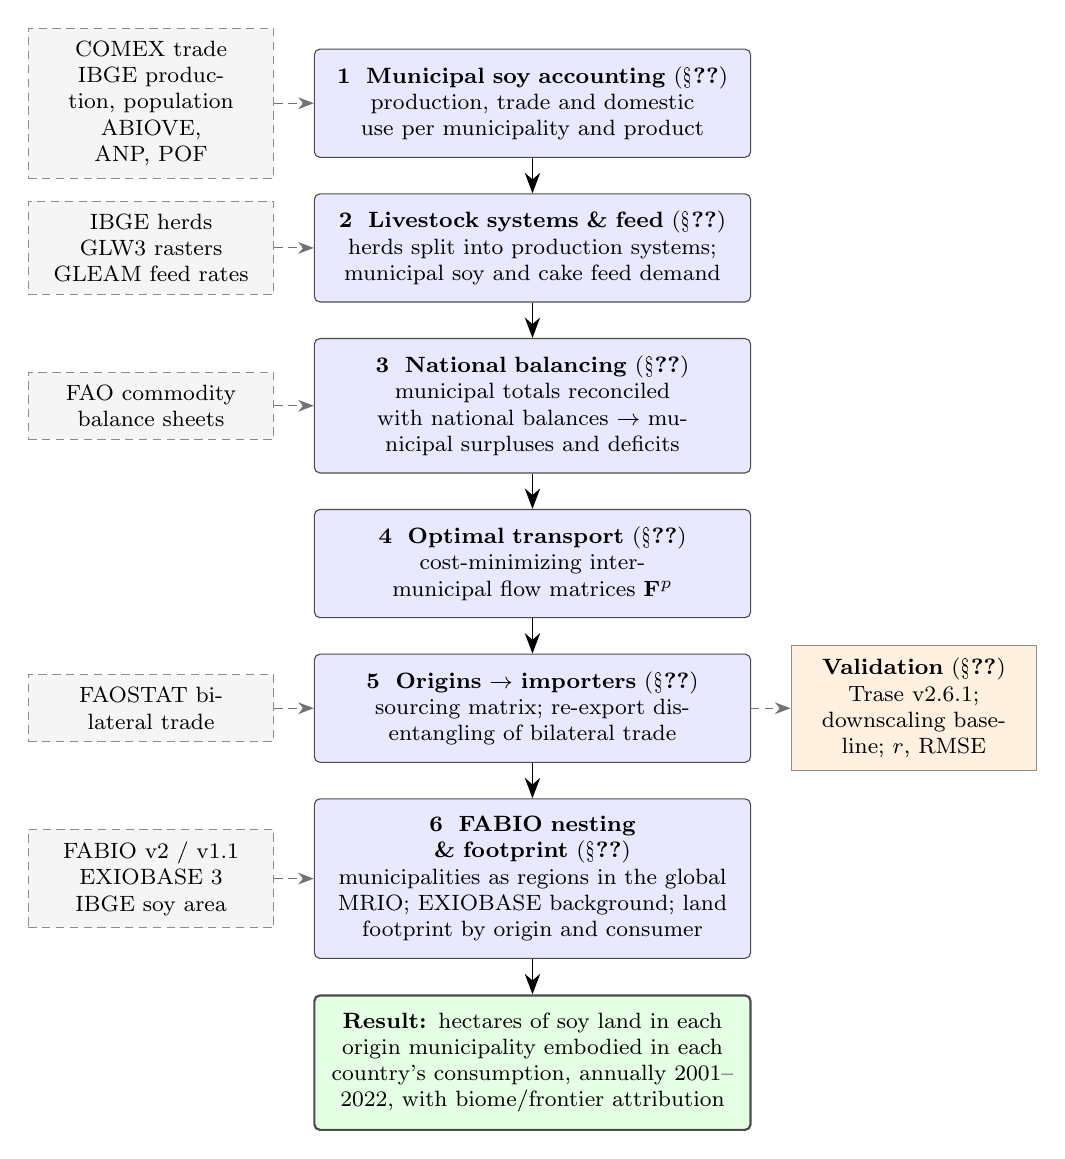
\begin{tikzpicture}[
  font=\footnotesize,
  stage/.style={draw=black!70, rounded corners=2pt, fill=blue!9,
                text width=51mm, align=center, inner sep=2.2mm},
  data/.style={draw=black!45, densely dashed, fill=black!4,
               text width=28mm, align=center, inner sep=1.6mm},
  res/.style={draw=black!70, thick, rounded corners=2pt, fill=green!10,
              text width=51mm, align=center, inner sep=2.2mm},
  val/.style={draw=black!45, fill=orange!12,
              text width=28mm, align=center, inner sep=1.6mm},
  arr/.style={-{Stealth[length=2.6mm]}, semithick},
  darr/.style={-{Stealth[length=2mm]}, densely dashed, black!55}
]
% --- main pipeline ---
\node[stage] (s1) {\textbf{1~~Municipal soy accounting}~(\S\ref{subsec:accounting})\\
  production, trade and domestic use per municipality and product};
\node[stage, below=4.5mm of s1] (s2) {\textbf{2~~Livestock systems \& feed}~(\S\ref{subsec:feed})\\
  herds split into production systems; municipal soy and cake feed demand};
\node[stage, below=4.5mm of s2] (s3) {\textbf{3~~National balancing}~(\S\ref{subsec:balancing})\\
  municipal totals reconciled with national balances $\rightarrow$
  municipal surpluses and deficits};
\node[stage, below=4.5mm of s3] (s4) {\textbf{4~~Optimal transport}~(\S\ref{subsec:transport})\\
  cost-minimizing inter-municipal flow matrices $\mathbf{F}^{p}$};
\node[stage, below=4.5mm of s4] (s5) {\textbf{5~~Origins $\rightarrow$ importers}~(\S\ref{subsec:origin2consumer})\\
  sourcing matrix; re-export disentangling of bilateral trade};
\node[stage, below=4.5mm of s5] (s6) {\textbf{6~~FABIO nesting \& footprint}~(\S\ref{subsec:fabio})\\
  municipalities as regions in the global MRIO; EXIOBASE background;
  land footprint by origin and consumer};
\node[res, below=4.5mm of s6] (out) {\textbf{Result:} hectares of soy land in each origin
  municipality embodied in each country's consumption, annually 2001--2022,
  with biome/frontier attribution};
% --- data inputs (left) ---
\node[data, left=5mm of s1] (d1) {COMEX trade\\ IBGE production, population\\ ABIOVE, ANP, POF};
\node[data, left=5mm of s2] (d2) {IBGE herds\\ GLW3 rasters\\ GLEAM feed rates};
\node[data, left=5mm of s3] (d3) {FAO commodity balance sheets};
\node[data, left=5mm of s5] (d5) {FAOSTAT bilateral trade};
\node[data, left=5mm of s6] (d6) {FABIO v2 / v1.1\\ EXIOBASE 3\\ IBGE soy area};
% --- validation (right) ---
\node[val, right=5mm of s5] (v) {\textbf{Validation}~(\S\ref{subsec:validation})\\
  Trase v2.6.1; downscaling baseline; $r$, RMSE};
% --- arrows ---
\draw[arr] (s1) -- (s2);
\draw[arr] (s2) -- (s3);
\draw[arr] (s3) -- (s4);
\draw[arr] (s4) -- (s5);
\draw[arr] (s5) -- (s6);
\draw[arr] (s6) -- (out);
\draw[darr] (d1) -- (s1);
\draw[darr] (d2) -- (s2);
\draw[darr] (d3) -- (s3);
\draw[darr] (d5) -- (s5);
\draw[darr] (d6) -- (s6);
\draw[darr] (s5) -- (v);
\end{tikzpicture}
\caption{Workflow of the study. Solid boxes are the six model stages
(Sections~\ref{subsec:accounting}--\ref{subsec:fabio}); dashed boxes are
the main data inputs at each stage; the orange box is the independent
validation of the reconstructed flows (Section~\ref{subsec:validation}).
Stages 1--5 reconstruct Brazil's subnational soy supply chain; stage 6 embeds
it in the global FABIO/EXIOBASE input--output framework and computes the
land-use footprint.}\label{fig:workflow}
\end{figure}

% ==================================================================
\subsection{Municipal soy accounting}\label{subsec:accounting}
% ==================================================================
In the first stage, a complete account of supply, trade and domestic use is
compiled for each Brazilian municipality for each of the three soy
products: soybeans, soy oil and soy cake (the protein meal remaining after
the beans are crushed for oil). Exports and imports are obtained from COMEX
customs records at municipality level, production data comes from IBGE
municipal surveys, and processing, storage and biodiesel infrastructure
data comes from ABIOVE, georeferenced warehouse registers and ANP. Each
item of the national FAO commodity balance for domestic use (crush, food,
seed, other uses (e.g.\ biodiesel) and stock changes) is then distributed
across municipalities according to the weight most closely tied to that use
(see Table~\ref{tab:weights}): installed crushing capacity for the crush,
household soy oil consumption for food use, and so on. The outcome is a
municipal supply--use account for beans, oil and cake that reproduces the
national commodity balance. \textcolor{green!50!black}{The
pipeline-specific processing choices and the treatment of stock
changes are detailed in Appendix~\ref{app:accounting}.}

\begin{table}[htbp]
\small
\caption{Domestic-use allocation: each item is a national commodity-balance
total distributed across municipalities in proportion to the stated weight
$w_m$ (Appendix~\ref{app:accounting}).}\label{tab:weights}
\begin{tabularx}{\textwidth}{@{}lX@{}}
\toprule
Use item & Allocation weight $w_m$ \\
\midrule
Processing (crush)  & installed crushing capacity \\
Food (beans, oil)   & per-capita soy-oil acquisition $\times$ population \\
Other (biodiesel)   & soy-attributable biodiesel capacity \\
Seed                & soybean production \\
Stock change        & storage capacity (beans), production (oil, cake); addition $\to$ use, withdrawal $\to$ supply \\
\botrule
\end{tabularx}
\end{table}

% ==================================================================
\subsection{Livestock systems and feed demand}\label{subsec:feed}
% ==================================================================
The next step is to estimate the municipal feed demand for soybeans and soy
cake. Since the amount of soy consumed by each animal varies greatly
depending on the livestock production system, the IBGE's herd counts at
municipal level are first divided into production systems (extensive,
intensive, and industrial monogastrics; grassland- and mixed-based
ruminants; dairy and meat) using the 2010 FAO gridded livestock maps (GLW3
and GLEAM). The number of animals in each system is then multiplied by the
amount of soy and soy cake consumed by each animal in that system, as
determined by GLEAM. The bottom-up totals are then rescaled to the national
feed use reported by the FAO (see Figure~\ref{fig:feed}). The outcome is
the municipal feed demand for beans and cake by species and production
system, which is consistent with the national balance. The
\textcolor{green!50!black}{splitting rules} and the implications of
keeping the 2010 system shares fixed
throughout the study period are provided in
Appendix~\ref{app:livestock}.

\begin{figure}[htbp]
\centering
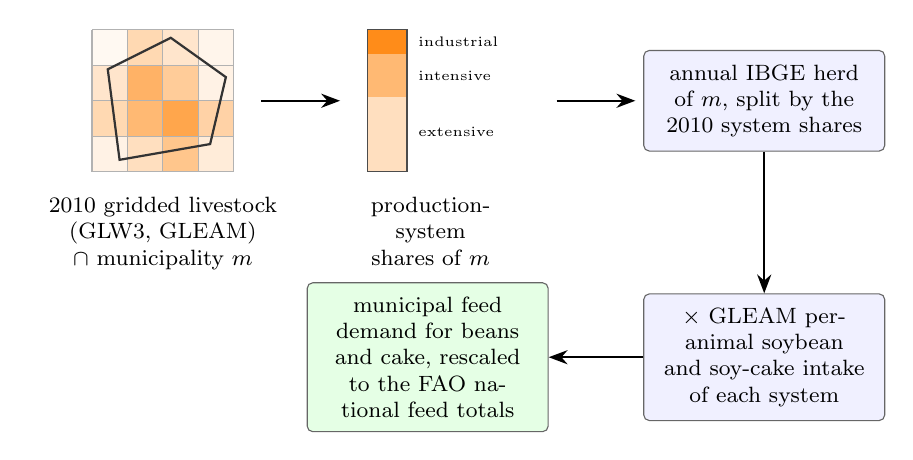
\begin{tikzpicture}[font=\footnotesize,
  box/.style={draw=black!60, rounded corners=2pt, fill=blue!6,
              text width=27mm, align=center, inner sep=1.8mm},
  arr/.style={-{Stealth[length=2.4mm]}, semithick}]
% --- raster with municipality polygon ---
\begin{scope}
\foreach \i/\j/\c in {0/0/10, 1/0/25, 2/0/45, 3/0/15,
                      0/1/30, 1/1/55, 2/1/70, 3/1/35,
                      0/2/20, 1/2/60, 2/2/40, 3/2/10,
                      0/3/5,  1/3/30, 2/3/20, 3/3/8}
  \fill[orange!\c] (\i*0.45,\j*0.45) rectangle (\i*0.45+0.45,\j*0.45+0.45);
\draw[black!30, step=0.45cm] (0,0) grid (1.8,1.8);
\draw[black!80, thick] (0.35,0.15) -- (1.5,0.35) -- (1.7,1.2)
  -- (1.0,1.7) -- (0.2,1.3) -- cycle;
\end{scope}
\node[below, text width=32mm, align=center] at (0.9,-0.2)
  {2010 gridded livestock (GLW3, GLEAM) $\cap$ municipality $m$};
\draw[arr] (2.15,0.9) -- (3.15,0.9);
% --- system-share bar ---
\begin{scope}[xshift=3.5cm]
\fill[orange!25] (0,0) rectangle (0.5,0.95);
\fill[orange!55] (0,0.95) rectangle (0.5,1.5);
\fill[orange!90] (0,1.5) rectangle (0.5,1.8);
\draw[black!70] (0,0) rectangle (0.5,1.8);
\node[right, font=\tiny] at (0.52,0.5)  {extensive};
\node[right, font=\tiny] at (0.52,1.22) {intensive};
\node[right, font=\tiny] at (0.52,1.65) {industrial};
\node[below, text width=24mm, align=center] at (0.8,-0.2)
  {production-system shares of $m$};
\end{scope}
\draw[arr] (5.9,0.9) -- (6.9,0.9);
% --- herd box ---
\node[box, anchor=west] (herd) at (7.0,0.9)
  {annual IBGE herd of $m$, split by the 2010 system shares};
% --- second row ---
\node[box, below=18mm of herd] (intake)
  {$\times$ GLEAM per-animal soybean and soy-cake intake of each system};
\node[box, fill=green!10, left=12mm of intake] (feed)
  {municipal feed demand for beans and cake, rescaled to the FAO national
   feed totals};
\draw[arr] (herd) -- (intake);
\draw[arr] (intake) -- (feed);
\end{tikzpicture}
\caption{From herds to municipal soy feed demand. Municipal herd counts
(annual) are divided into production systems using the shares implied by
the 2010 gridded livestock rasters within each municipality. Each system's
herd is multiplied by its per-animal soy and soy-cake intake, and the
totals are then scaled to match the national feed use reported by the
FAO.}\label{fig:feed}
\end{figure}

% ==================================================================
\subsection{National balancing}\label{subsec:balancing}
% ==================================================================
Next, the municipal accounts are reconciled with the national supply--use
identity of each product (production $+$ imports $+$ stock withdrawal $=$
exports $+$ food $+$ feed $+$ seed $+$ processing $+$ other). Municipal
trade is harmonised with the FABIO/FAOSTAT bilateral trade classification.
Any remaining national residual is absorbed into the stock term and each
balance item is proportionally rescaled so that every municipal aggregate
matches its national total exactly. The outcome is a balanced set of
municipal net positions for each product (a surplus where local supply
exceeds use, a deficit where use exceeds supply). The supply--use identity,
the surplus/deficit decomposition, and the treatment of net stock
withdrawals are explained in Appendix~\ref{app:balancing}.

% ==================================================================
\subsection{Subnational transport allocation}\label{subsec:transport}
% ==================================================================
In this step, municipal surpluses and deficits are connected via optimal
transport that minimises costs. For each product, the inter-municipal flow
matrix $\mathbf{F}^p$ is the cheapest way to assign surpluses to deficits
while conserving mass. The premise is that bulk-commodity logistics
minimise freight costs, which increase with distance. Three allocation
variants are analysed in order of increasing supply-chain structure: a
pure downscaling baseline, which ignores the domestic network and
splits each destination's imports across municipalities according to their
production shares; the Euclidean model, which solves the
transportation problem using straight-line distances between municipal
centres; and a multimodal variant, which uses Brazil's actual road,
rail and waterway networks for the same flows, taking into account
mode-specific freight costs and corridor capacities (all three variants
are specified in Appendix~\ref{app:transport}). When compared with the
independent Trase benchmark, the three models produce similar results at
the aggregate level: the pooled municipality$\times$destination
correlation averages 0.71, 0.69 and 0.69 respectively over the period from
2010 to 2022, but differences emerge at the level of individual
destinations (see Section~\ref{subsec:validation}). The reported results
use the Euclidean model: the multimodal variant does not reproduce the
benchmark better than the Euclidean model in any year, and requires
network inputs that are unavailable for parts of the study period. The
downscaling baseline produces no inter-municipal flows, which are required
for the tracing of processing, feed and domestic consumption in stage~5.
The outcome is a deterministic inter-municipal flow
matrix per product whose margins reproduce the municipal surpluses and
deficits by construction. \textcolor{green!50!black}{The formal
problem statement and the solvers are specified in
Appendix~\ref{app:transport}; the multimodal benchmark results are
reported in Section~\ref{subsec:validation}.}

% ==================================================================
\subsection{From origins to consumers}\label{subsec:origin2consumer}
% ==================================================================
The COMEX customs records of stage~1 attach two labels to every exported
tonne: the municipality that shipped it and the country that first
imported it. However, neither label contains the information that the
footprint needs: the municipality that grew the soy and the country that
finally consumes it. This stage corrects both issues. Within Brazil, the
transport flows of stage~4 serve as the tracing device. Completed with
each municipality's retained supply, they yield sourcing shares that trace
every exported (and domestically consumed) tonne back to its origin
municipality (Figure~\ref{fig:tracing}). Oil and cake are traced one step
further back to the municipalities where the beans were grown. Moving
forwards across borders, exported tonnes often pass through intermediate
countries before being consumed. The FAOSTAT bilateral trade data are
therefore corrected for re-exports \cite{kastner2011tracing}: each tonne
is followed through the trade network until it reaches the country where
it is finally consumed (Figure~\ref{fig:tracing}). In this calculation,
Brazil enters as its individual municipalities rather than as a single
country. The outcome is an origin-to-consumption matrix linking every
producing municipality to every consuming country. The equations, the
underlying proportional-mixing assumption and its numerical implementation
are given in Appendix~\ref{app:tracing}.

\begin{figure}[htbp]
\centering
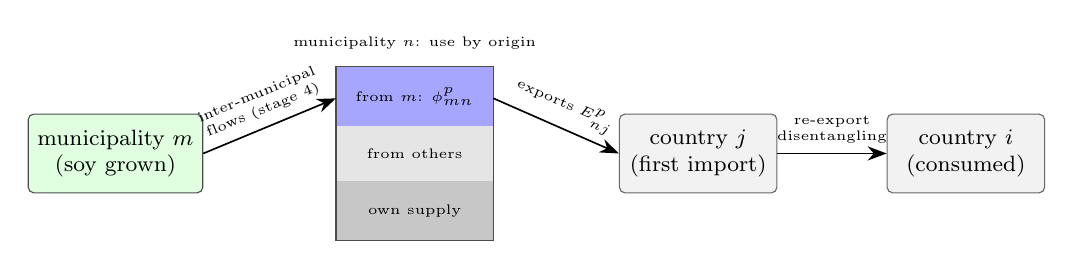
\begin{tikzpicture}[font=\footnotesize,
  mun/.style={draw=black!70, rounded corners=2pt, fill=green!12,
              minimum width=20mm, minimum height=10mm, align=center},
  cty/.style={draw=black!60, rounded corners=2pt, fill=black!5,
              minimum width=20mm, minimum height=10mm, align=center},
  lab/.style={font=\tiny, align=center},
  arr/.style={-{Stealth[length=2.4mm]}, semithick}]
% --- origin municipality m ---
\node[mun] (m) at (0,0.4) {municipality $m$\\ (soy grown)};
% --- municipality n: use divided by origin ---
\fill[blue!35]  (2.8,0.75) rectangle (4.8,1.50);   % the part from m
\fill[black!10] (2.8,0.05) rectangle (4.8,0.75);   % from other municipalities
\fill[black!22] (2.8,-0.70) rectangle (4.8,0.05);  % own supply of n
\draw[black!70] (2.8,-0.70) rectangle (4.8,1.50);
\node[lab] at (3.8,1.125) {from $m$: $\phi^p_{mn}$};
\node[lab] at (3.8,0.40)  {from others};
\node[lab] at (3.8,-0.325) {own supply};
\node[lab, anchor=south] at (3.8,1.60) {municipality $n$: use by origin};
% --- countries ---
\node[cty] (j) at (7.4,0.4) {country $j$\\ (first import)};
\node[cty] (i) at (10.8,0.4) {country $i$\\ (consumed)};
% --- arrows ---
\draw[arr] (m.east) -- node[lab, above, sloped] {inter-municipal\\ flows (stage~4)} (2.8,1.1);
\draw[arr] (4.8,1.1) -- node[lab, above, sloped] {exports $E^p_{nj}$} (j.west);
\draw[arr] (j.east) -- node[lab, above] {re-export\\ disentangling} (i.west);
\end{tikzpicture}
\caption{Tracing a tonne from origin to final consumer. The soy grown in
municipality $m$ reaches municipality $n$ through the inter-municipal
flows of stage~4, so the share $\phi^p_{mn}$ of $n$'s use is attributed
to $m$ (highlighted). The observed exports $E^p_{nj}$ of $n$ carry that
share to the country of first import $j$, and the re-export disentangling
reattributes it to the country of final consumption $i$. The corresponding
equations are given in Appendix~\ref{app:tracing}.}\label{fig:tracing}
\end{figure}

% ==================================================================
\subsection{Nesting into FABIO and footprint accounting}\label{subsec:fabio}
% ==================================================================
In the final stage, the reconstructed municipal soy economy is embedded in
the FABIO physical MRIO, in which a process is a
region$\times$commodity unit. Brazil's three national soy commodities and
processes are removed and replaced by their $\sim$16{,}700 municipal
counterparts, so that municipalities enter the global model as additional
regions, each carrying its own production, soy area, feed use and
origin-resolved trade from the previous stages (Figure~\ref{fig:nesting}).
The regional accounts are then linked through the re-export-corrected
trade of stage~5 into a single global input--output model, following the
published FABIO procedure \cite{bruckner2019fabio}. Soy used outside the
food system, for example as biodiesel, is traced onwards by coupling FABIO
to the EXIOBASE model of the wider economy \cite{stadler2018exiobase}.
From 2010 onwards the model runs on the FABIO
v2 backend; for 2001--2009 it switches to inputs from the FABIO v1.1 build,
and the seam between the two backends is quantified on the overlap years
2010--2013. \textcolor{green!50!black}{The backend bridging and seam
analysis are documented in Appendix~\ref{app:nesting}; the assembly of
the nested model and the EXIOBASE coupling follow the published FABIO
procedures \cite{bruckner2019fabio,stadler2018exiobase}.}

\begin{figure}[htbp]
\centering
% --- panel a: how municipal Brazil is inserted into the FABIO process list ---
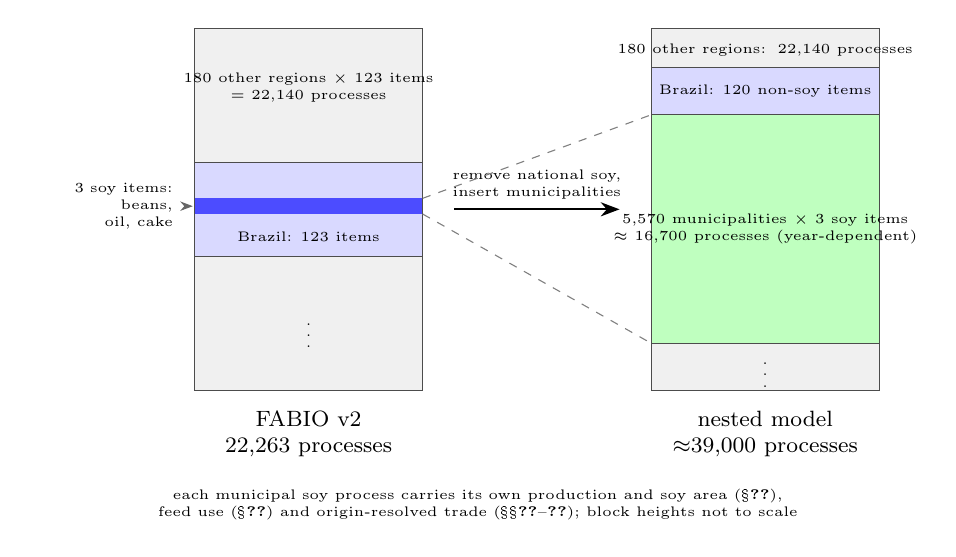
\begin{tikzpicture}[font=\footnotesize,
  arr/.style={-{Stealth[length=2.4mm]}, semithick},
  brc/.style={decorate, decoration={brace, amplitude=3pt}, black!60},
  dimlab/.style={font=\tiny, black!70, align=left}]
% ---- left column: original FABIO process list ----
\draw[fill=black!6, draw=black!70] (0,0) rectangle (2.9,4.6);
\fill[blue!15] (0,1.7) rectangle (2.9,2.9);
\fill[blue!70] (0,2.24) rectangle (2.9,2.44); % national soy stripe
\draw[black!70] (0,1.7) rectangle (2.9,2.9);
\node[font=\tiny, align=center] at (1.45,3.85)
  {180 other regions $\times$ 123 items\\ $=$ 22{,}140 processes};
\node[font=\tiny] at (1.45,1.95) {Brazil: 123 items};
\node[font=\tiny] at (1.45,0.8) {\vdots};
\node[font=\tiny, anchor=east, align=right, text width=15mm] at (-0.15,2.34)
  {3 soy items: beans, oil, cake};
\draw[-{Stealth[length=1.6mm]}, black!60] (-0.12,2.34) -- (-0.02,2.34);
\node[align=center] at (1.45,-0.55) {FABIO v2\\ 22{,}263 processes};
% ---- arrow ----
\draw[arr] (3.3,2.3) -- node[above, align=center, text width=22mm, font=\tiny]
  {remove national soy, insert municipalities} (5.4,2.3);
% ---- right column: nested process list ----
\draw[fill=black!6, draw=black!70] (5.8,0) rectangle (8.7,4.6);
\fill[blue!15] (5.8,3.5) rectangle (8.7,4.1);
\draw[black!70] (5.8,3.5) rectangle (8.7,4.1);
\fill[green!25] (5.8,0.6) rectangle (8.7,3.5);
\draw[black!70] (5.8,0.6) rectangle (8.7,3.5);
\node[font=\tiny, align=center] at (7.25,4.32) {180 other regions:\, 22{,}140 processes};
\node[font=\tiny, align=center] at (7.25,3.8) {Brazil: 120 non-soy items};
\node[font=\tiny, align=center] at (7.25,2.05)
  {5{,}570 municipalities $\times$ 3 soy items\\ $\approx$ 16{,}700 processes (year-dependent)};
\node[font=\tiny] at (7.25,0.3) {\vdots};
\node[align=center] at (7.25,-0.55) {nested model\\ $\approx$39{,}000 processes};
% zoom lines from national soy stripe to municipal block
\draw[dashed, black!50] (2.9,2.44) -- (5.8,3.5);
\draw[dashed, black!50] (2.9,2.24) -- (5.8,0.6);
% data provenance (below panel)
\node[align=center, font=\tiny, text width=112mm] at (3.6,-1.45)
  {each municipal soy process carries its own production and soy area
   (\S\ref{subsec:accounting}), feed use (\S\ref{subsec:feed}) and
   origin-resolved trade
   (\S\S\ref{subsec:transport}--\ref{subsec:origin2consumer});
   block heights not to scale};
\end{tikzpicture}

\caption{Nesting municipal soy into the global input--output system: the
three national Brazilian soy commodities are removed from the process list
and replaced by one soy process set per municipality, populated with the
municipal accounts of stages 1--5; all other regions, and Brazil's
remaining commodities, are untouched. \textcolor{green!50!black}{The
assembly follows the published FABIO procedure
\cite{bruckner2019fabio}; the backend coverage and the seam analysis
are detailed in Appendix~\ref{app:nesting}.}}\label{fig:nesting}
\end{figure}

\paragraph{Land-use footprint accounting.}\label{subsec:footprint}
The direct land use of each process is its harvested soy area, taken from
IBGE for the municipal soy processes and from the FABIO land-use extension
for all others. Dividing by output gives a land intensity per unit of
product, which the footprint calculation traces through the supply chains
to each country's final demand, food and non-food uses alike. Each
municipality is assigned to a biome (IBGE 1:250{,}000 layer), and the
agricultural frontier is defined as the Amazon biome plus MATOPIBA. The
result is hectares of soy land in each origin municipality embodied in
each country's consumption, per year, with biome and frontier attribution.
The treatment of stocks, footprints by consumed product, and the optional
30\,m grid refinement are described in Appendix~\ref{app:footprint}.

% ==================================================================
\subsection{Headline results}\label{subsec:highlights}
% ==================================================================
Four outputs illustrate what the pipeline delivers. The footprint grew
from 9.4~Mha in 2001 to 41.0~Mha in 2022, with its origin shifting from
the southern states to the Cerrado frontier (see Fig.~\ref{fig:maps}).
During the same period, the EU-27 and China exchanged roles as the
dominant consumer, with this change occurring in 2009--2010
(Fig.~\ref{fig:destination}). Most of the footprint reaches consumers in
commodity form. From 2010 onwards, around a quarter is embodied in animal
products (Fig.~\ref{fig:enduse}). At the finest level, the footprint can
be displayed as probability maps per destination on 30\,m MapBiomas soy
pixels (Fig.~\ref{fig:probmaps}).

\begin{figure}[H]
\centering
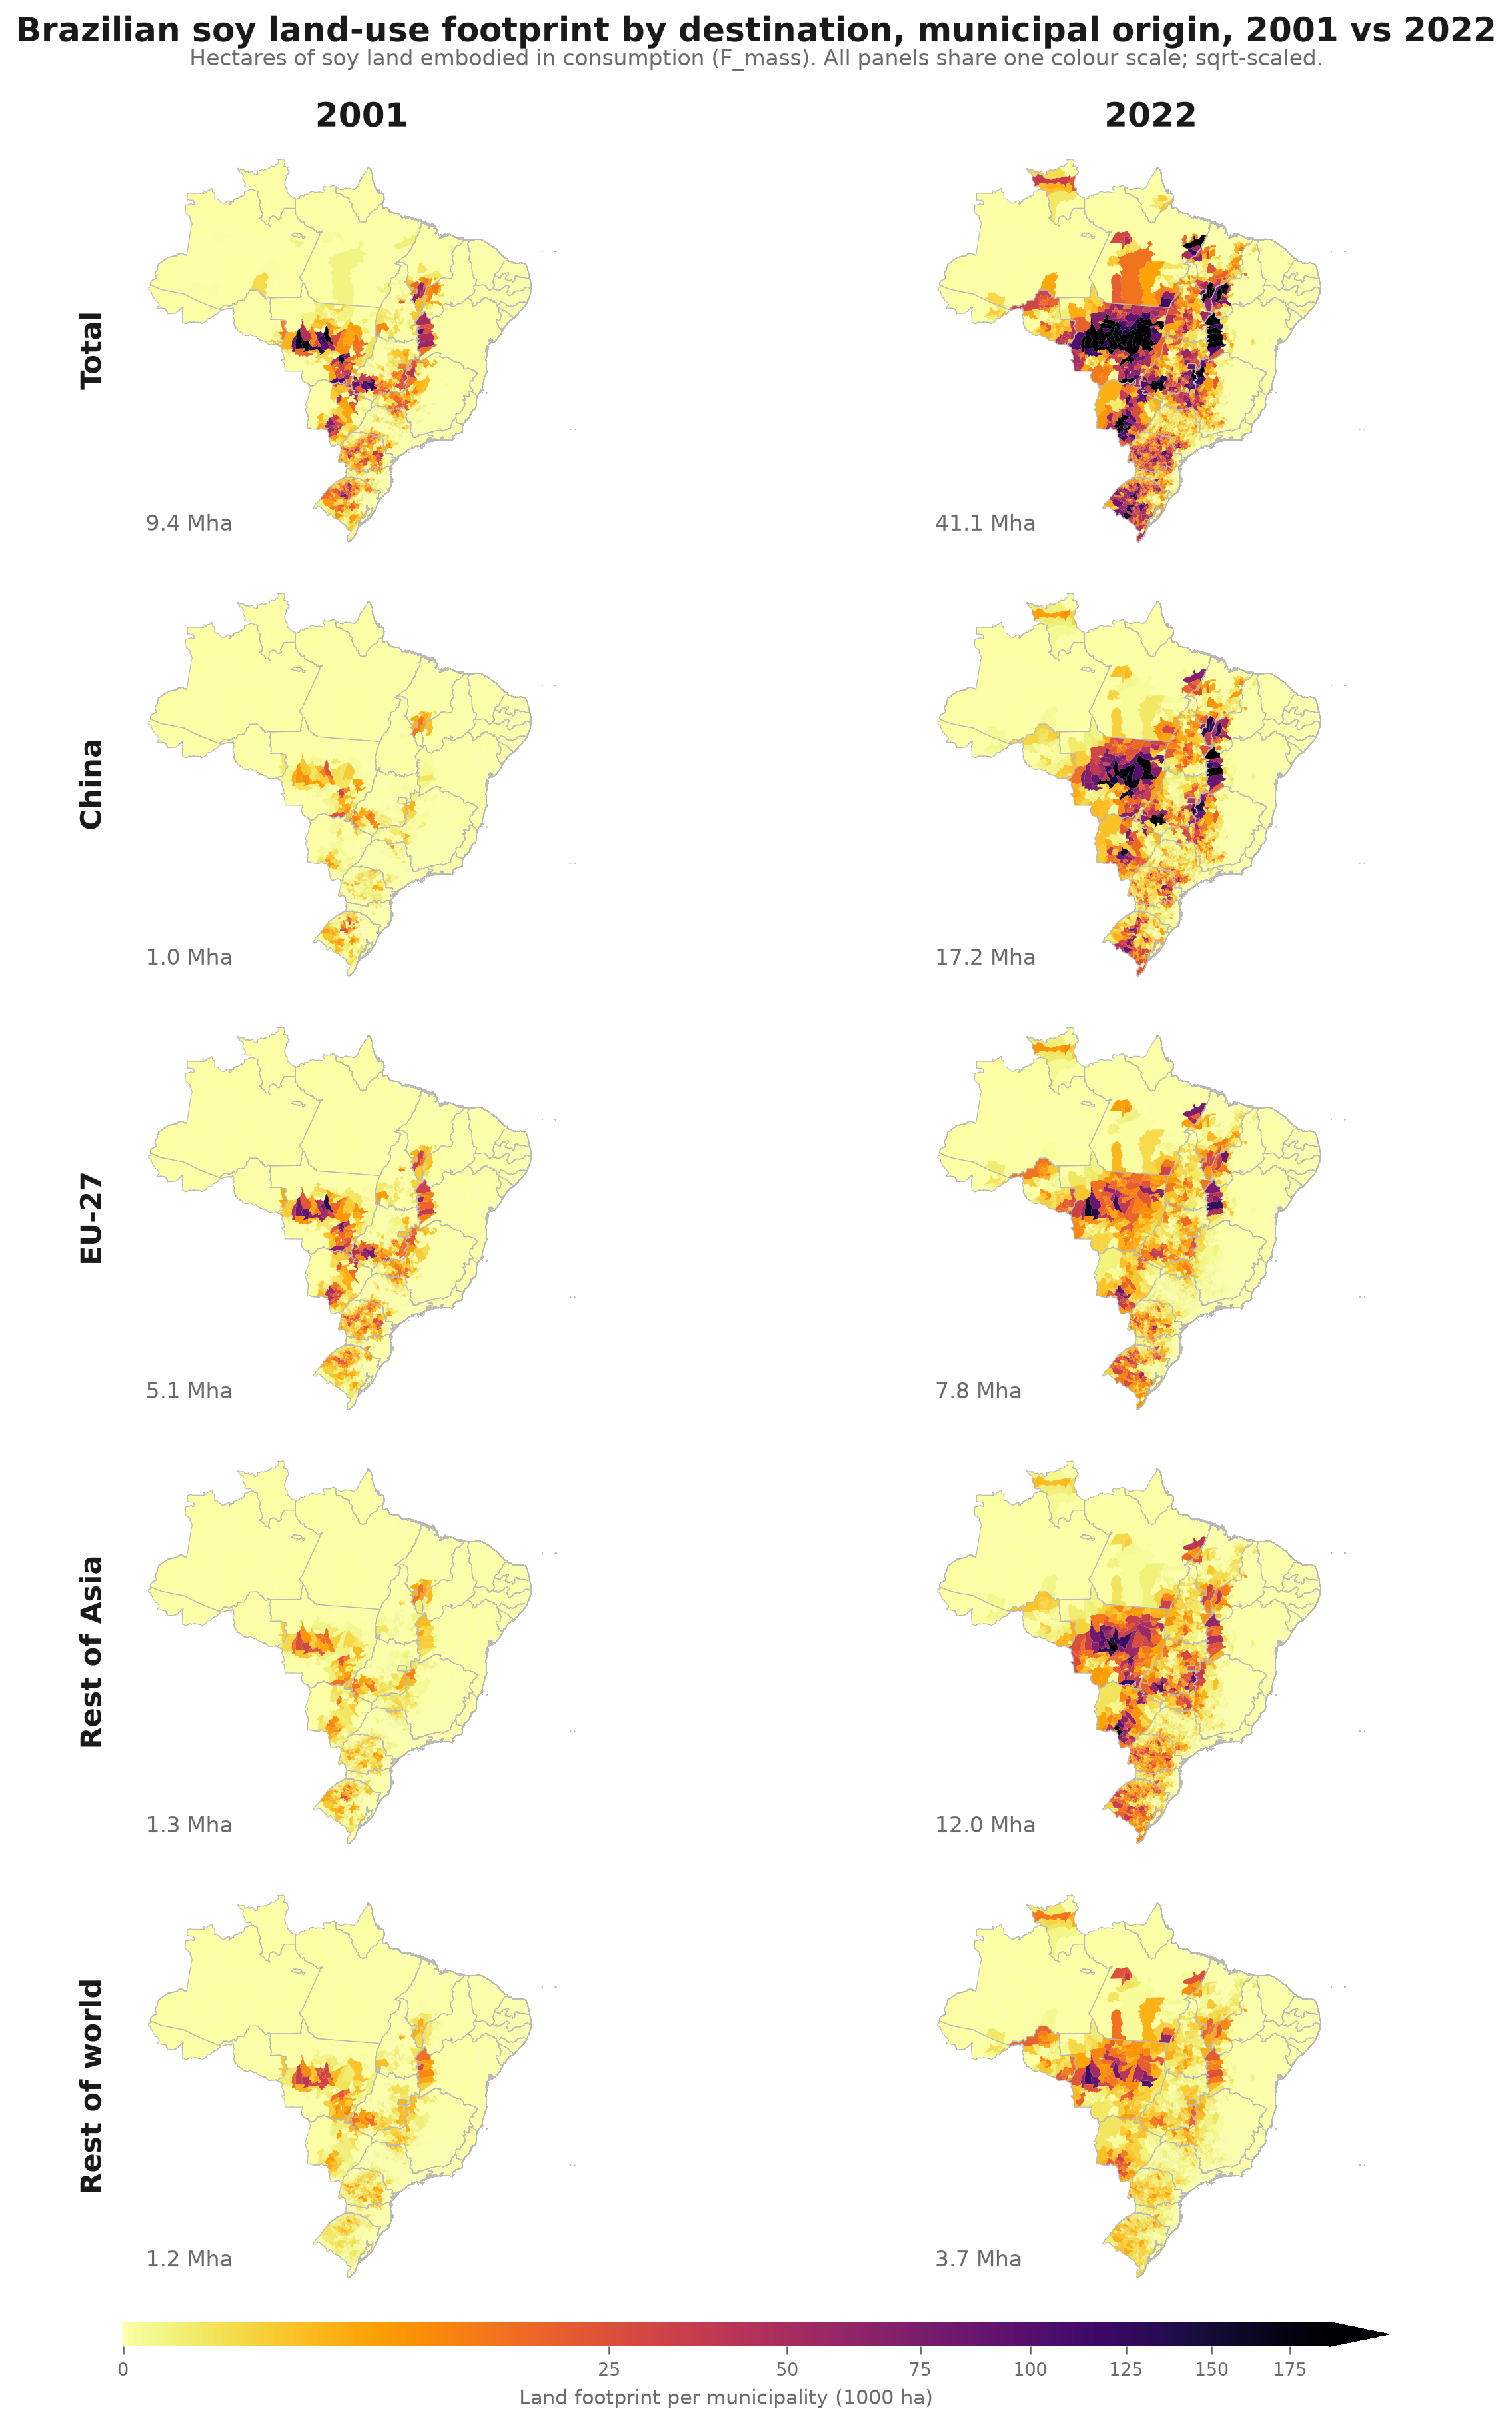
\includegraphics[width=\textwidth,height=0.94\textheight,keepaspectratio]{figures/map_2001_2022.png}
\caption{Municipal origin of the Brazilian soy land-use footprint, 2001
versus 2022, for the total and the four major destination groups; all
panels share one square-root colour scale. An interactive year-by-year
version is available at
\url{https://lizaburiak.github.io/soyprint-footprint-map/}.}
\label{fig:maps}
\end{figure}

\begin{figure}[H]
\centering
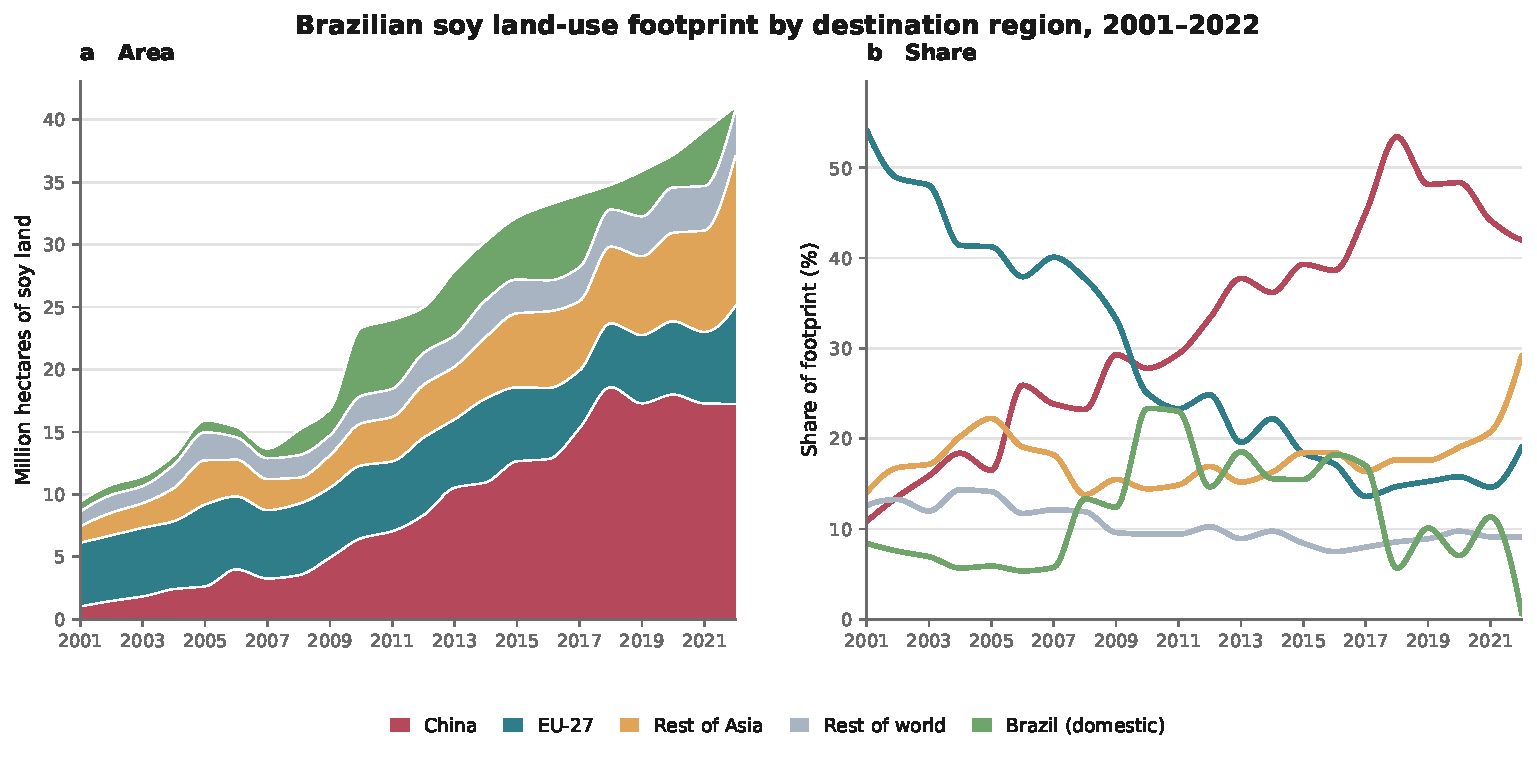
\includegraphics[width=\textwidth]{figures/fig_by_destination.pdf}
\caption{Footprint by destination region, 2001--2022: (a)~absolute
footprint, (b)~regional shares.}\label{fig:destination}
\end{figure}

\begin{figure}[H]
\centering
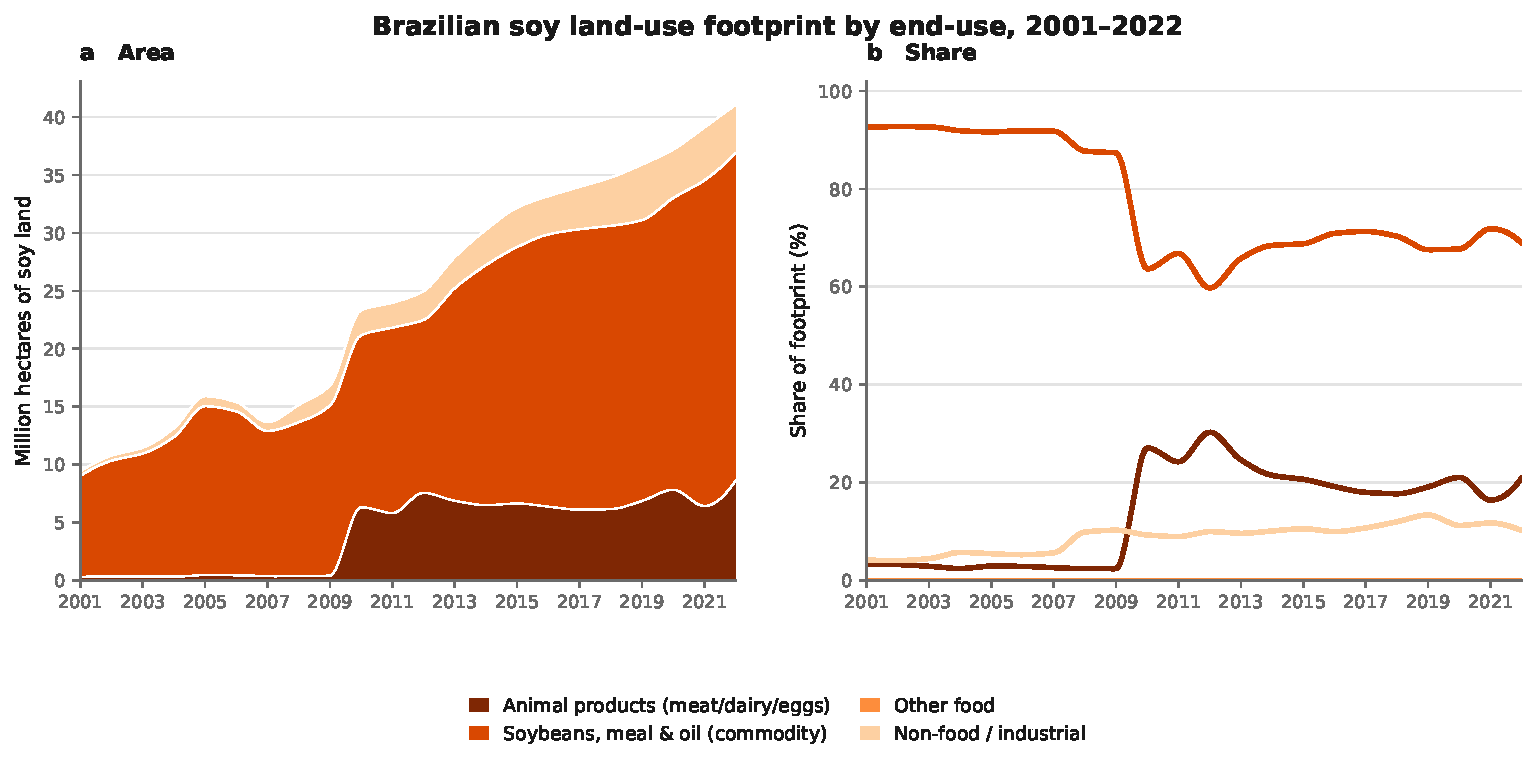
\includegraphics[width=\textwidth]{figures/fig_enduse.pdf}
\caption{Footprint by end-use, 2001--2022: (a)~absolute footprint,
(b)~end-use shares.}\label{fig:enduse}
\end{figure}

\begin{figure}[H]
\centering
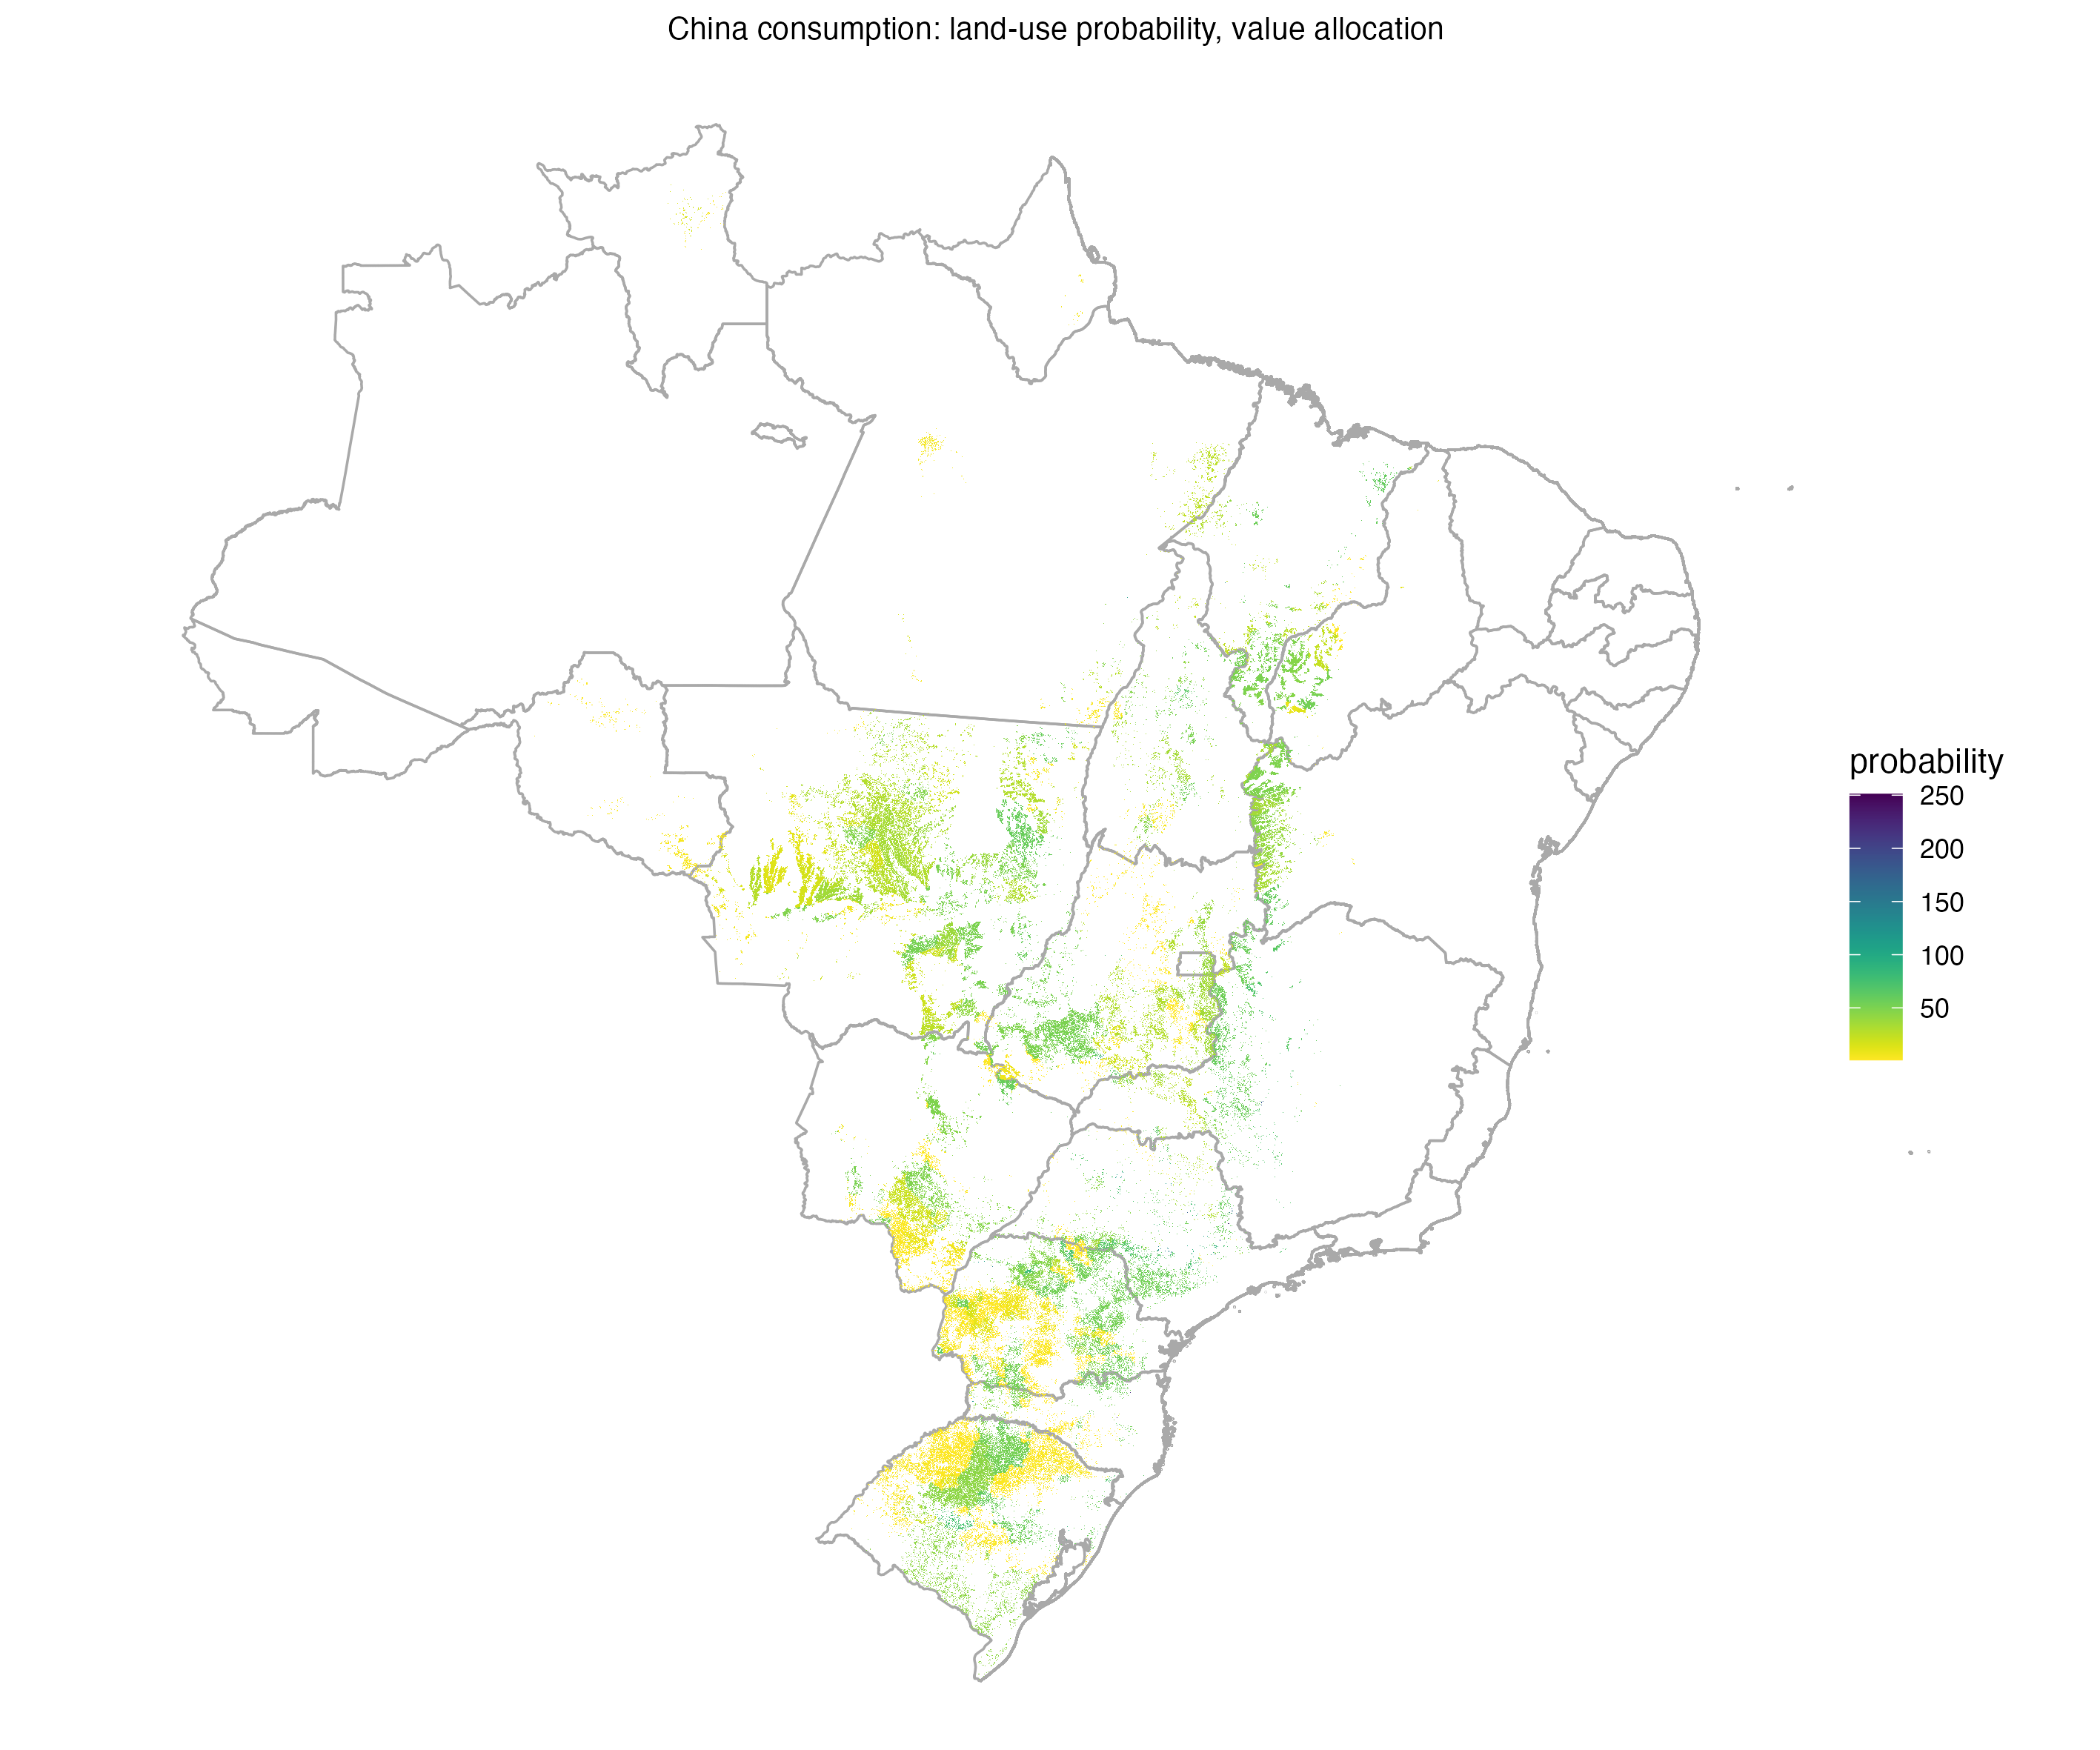
\includegraphics[width=0.49\textwidth]{figures/prob_map_china_2022.png}\hfill
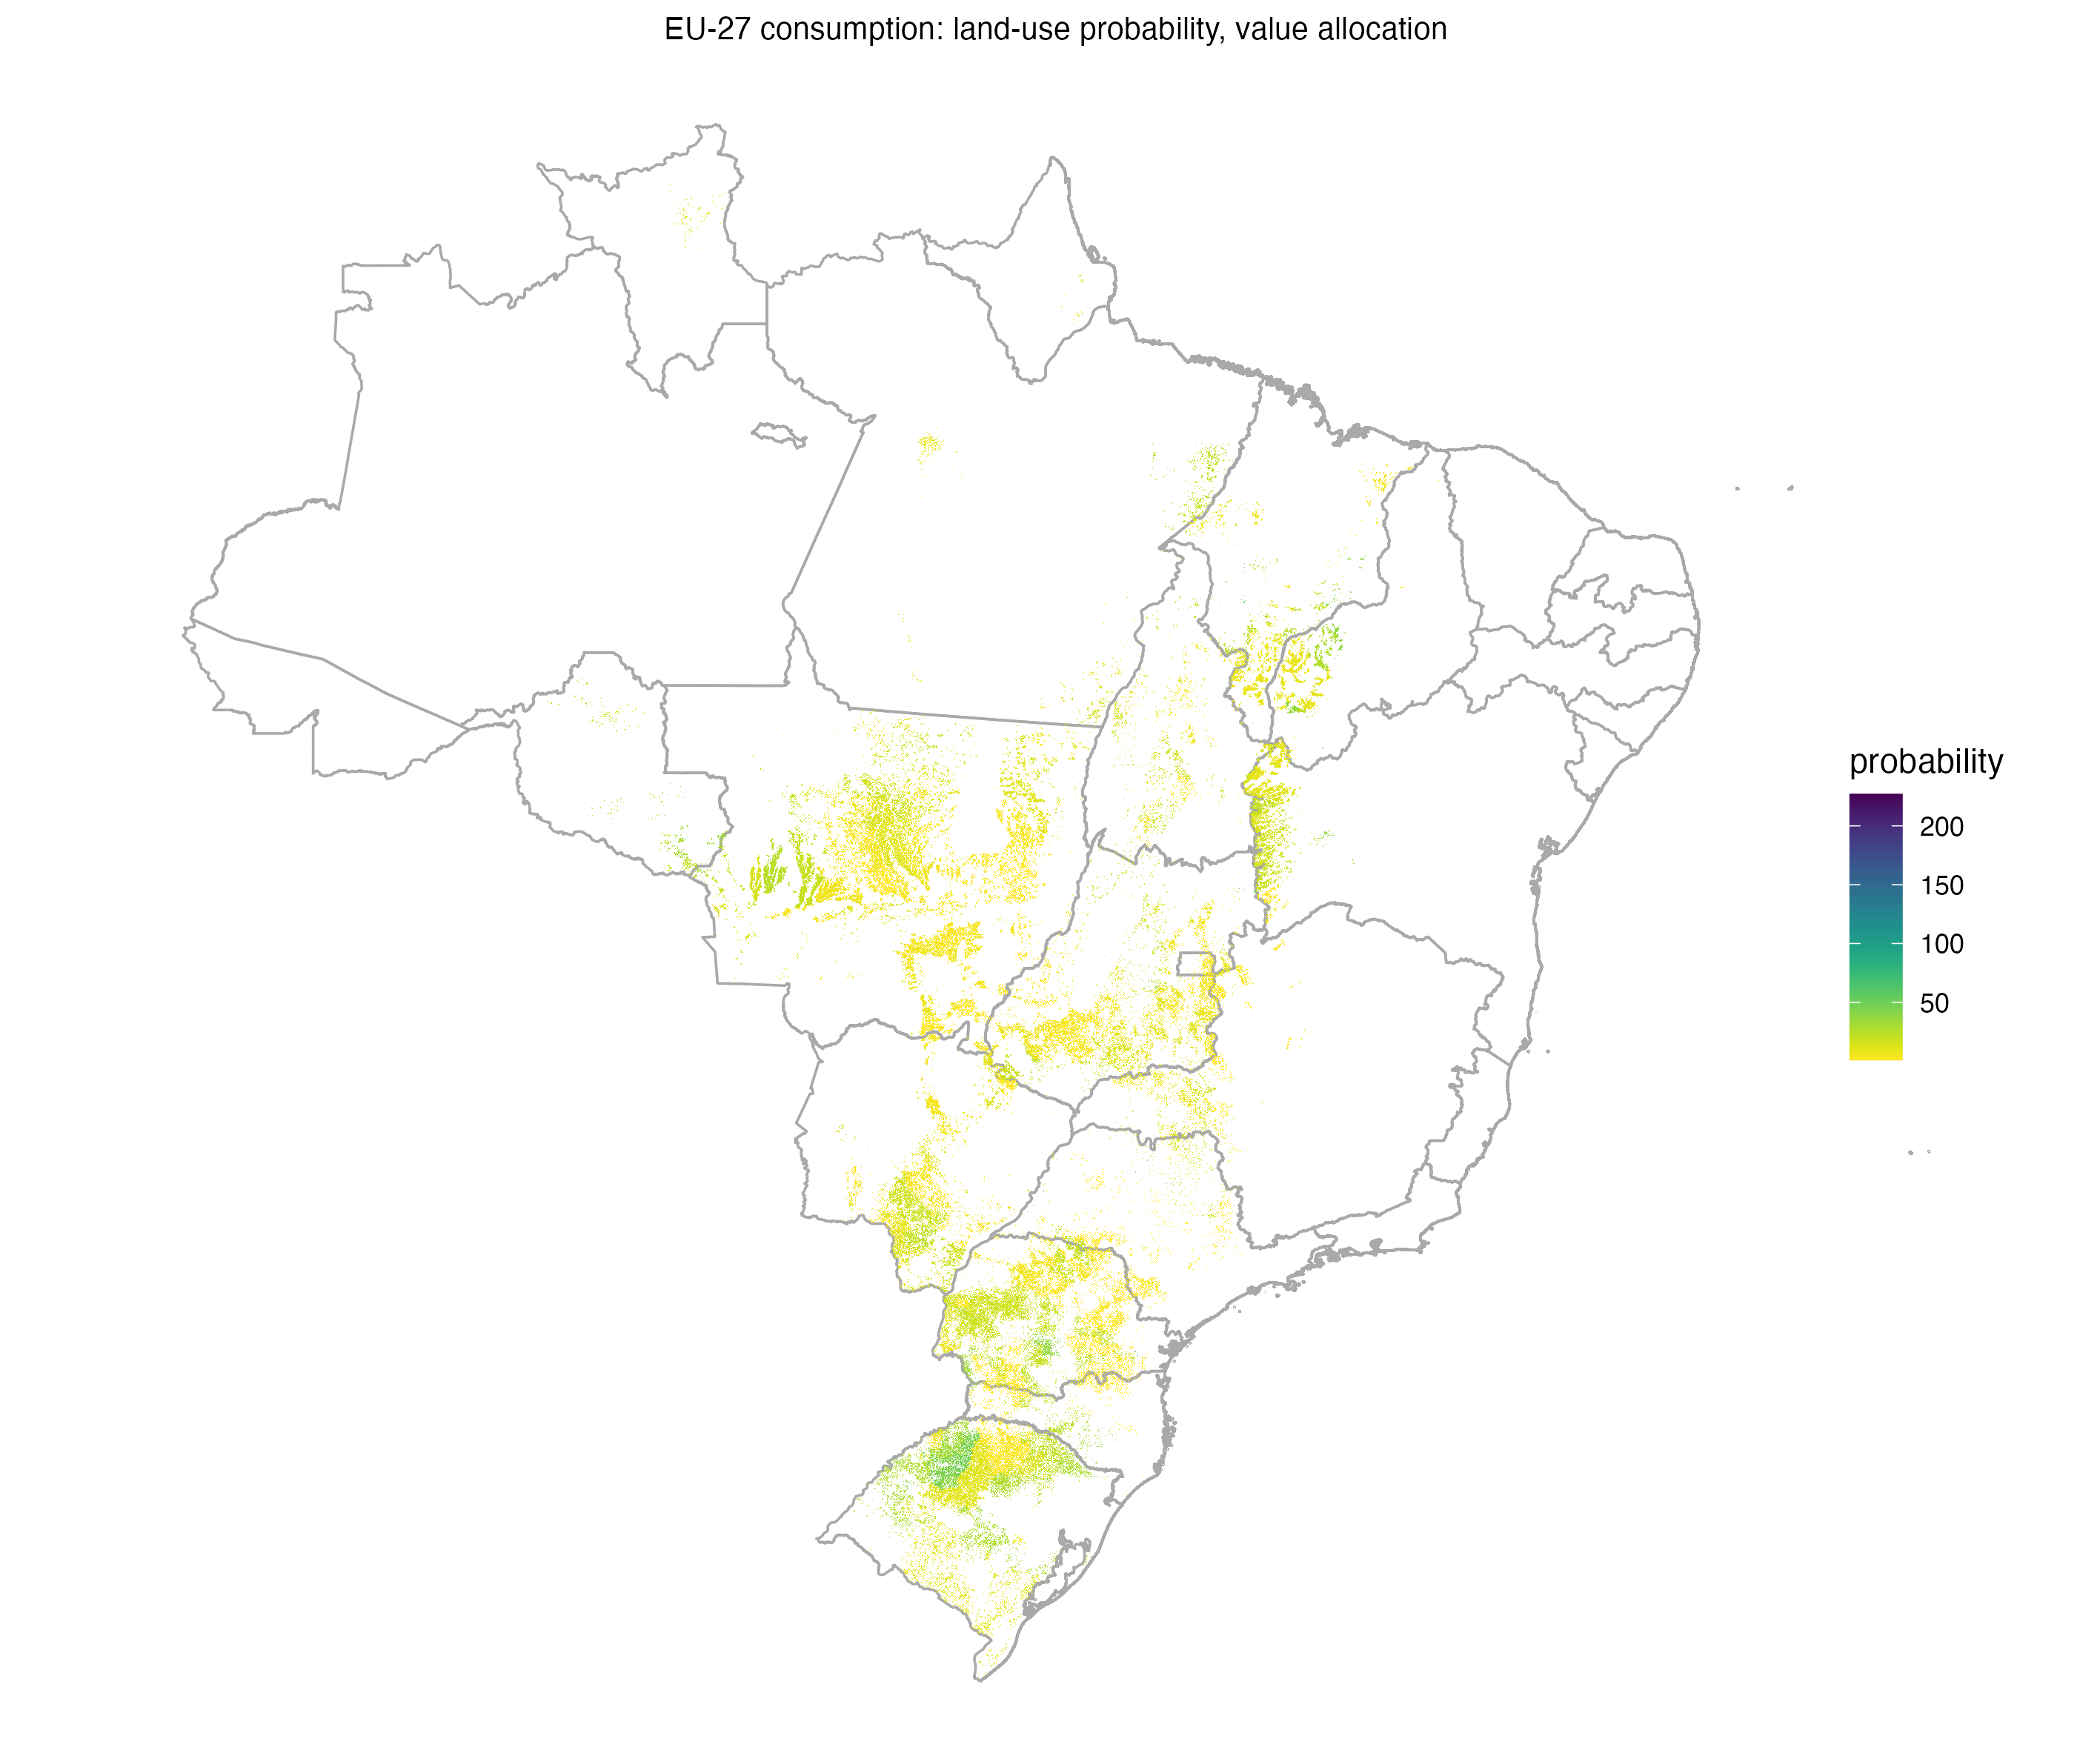
\includegraphics[width=0.49\textwidth]{figures/prob_map_eu27_2022.png}
\caption{Probability maps of the 2022 footprint on 30\,m MapBiomas soy
pixels, for China (left) and the EU-27 (right); colour gives the pixel's
probability of serving the destination's consumption (value
allocation).}\label{fig:probmaps}
\end{figure}

% ==================================================================
\subsection{Validation and uncertainty}\label{subsec:validation}
% ==================================================================
The reconstructed origin-to-importer flows are evaluated against the
independent Trase Brazil--soy dataset (v2.6.1), which links municipalities
of production to countries of first import using per-shipment customs and
logistics records \cite{godar2015sei,escobar2020trase}. All three
allocation variants of Section~\ref{subsec:transport} are compared
against this benchmark on the municipality$\times$destination flow
matrix: the downscaling baseline, the Euclidean model and the multimodal
variant (Figure~\ref{fig:models}). Pooled over all flows the three
perform comparably, with mean correlations of 0.71, 0.69 and 0.69 over
2010--2022. The value added by the supply-chain structure shows at the
destination level: the mean per-destination correlation is 0.41 for the
Euclidean model and 0.42 for the multimodal variant, against 0.28 for
downscaling. \textcolor{green!50!black}{Sample construction is given
in Appendix~\ref{app:validation}.}

\begin{figure}[H]
\centering
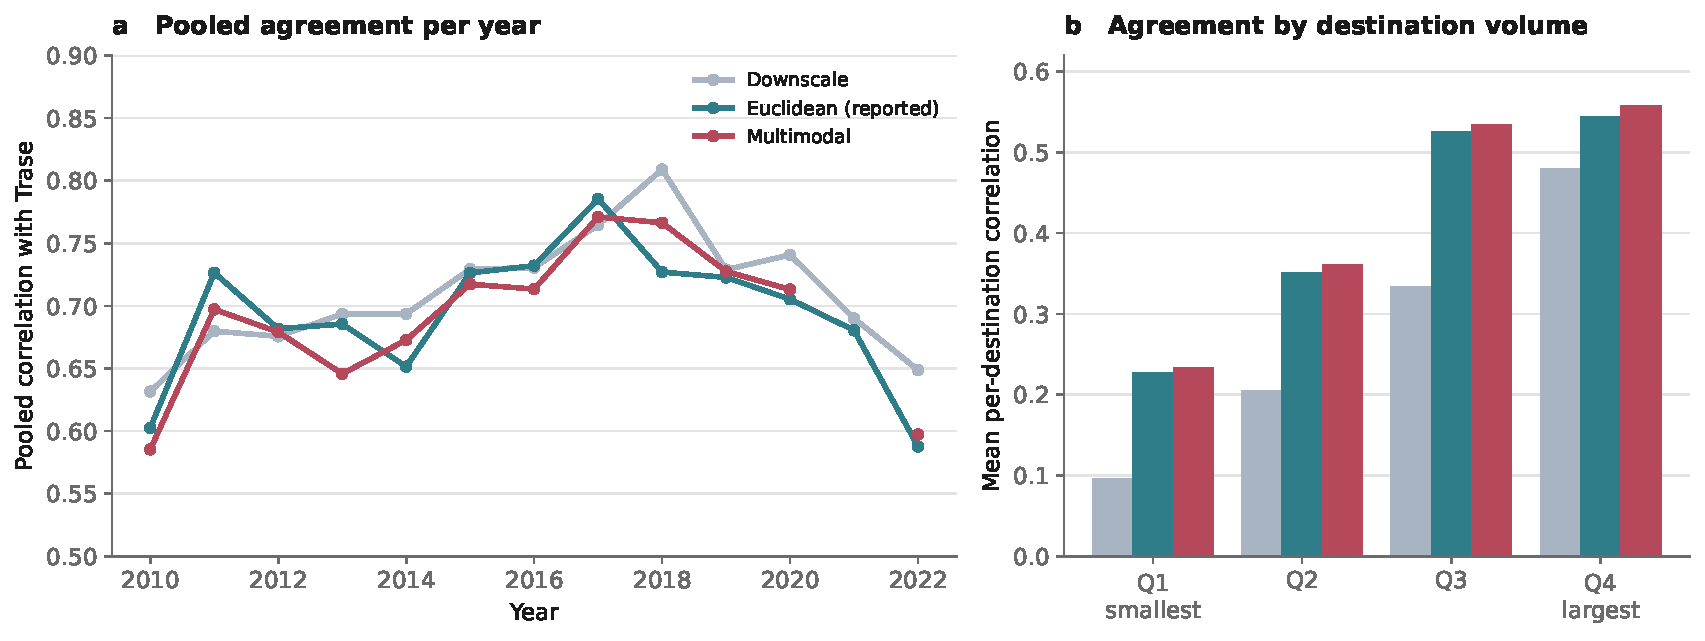
\includegraphics[width=\textwidth]{figures/fig_model_comparison.pdf}
\caption{The three allocation variants against the Trase benchmark,
2010--2022. (a)~Pooled municipality$\times$destination correlation per
year (the multimodal variant has no 2021 solve). (b)~Mean per-destination
correlation by import-volume quartile: the supply-chain models separate
from downscaling at the destination level, and all variants improve with
volume.}\label{fig:models}
\end{figure}

Agreement rises with flow size (Figure~\ref{fig:rocket}). Pooled over
the \textcolor{green!50!black}{91{,}873} matched
municipality$\times$destination$\times$year
flows \textcolor{green!50!black}{of 2010--2022}, the log-flow
correlation with Trase is 0.68 and 54\% of the flows
fall within a factor of three of the benchmark value. In the upper half
of the volume distribution (flows above 1.2\,kt, which carry 98\% of
the benchmark tonnage) the within-factor-three share rises to
\textcolor{green!50!black}{57\%} and
the median deviation falls from a factor of
\textcolor{green!50!black}{2.6 to 2.3}; per destination,
the mean correlation rises from 0.29 in the lower half of import volumes
to 0.53 in the upper half. The tonnage that carries the footprint is
therefore also the best-validated part of the flow distribution, and
below roughly $10^3$\,t per destination subnational modelling adds no
information over downscaling (Appendix~\ref{app:validation}).

\begin{figure}[H]
\centering

\includegraphics[width=0.94\textwidth]{figures/rocket_plot_years.pdf}
\caption{Agreement with the benchmark grows with flow size (``rocket
plots''). Every modelled municipality$\times$destination soy export flow is
plotted against the corresponding Trase flow (both $\log_{10}$ tonnes;
flows below 1\,t on either side are excluded) for four sample years, with
\textcolor{green!50!black}{density contours} and the 1:1 line (dashed); each panel reports the
number of matched flows, the log-scale Pearson correlation and the share of
flows agreeing within a factor of three. Large flows converge onto the 1:1
diagonal (the ``nose''), while small flows scatter (the ``plume''):
agreement rises systematically with volume, which motivates the volume
floor of the decision rule (Appendix~\ref{app:validation}): the tonnage
that carries the footprint is also the best-validated part of the flow
distribution.}\label{fig:rocket}
\end{figure}

A second, temporal check concerns the two FABIO backends. Before 2010 the
pipeline runs on FABIO v1.1 inputs instead of the v2 build
(Section~\ref{subsec:fabio}); in the clean overlap years the two
backends differ by 6--8\% in the total footprint with cross-country
correlations above 0.988, so pre-2010 levels are reported unadjusted
(Appendix~\ref{app:nesting}).

\textcolor{green!50!black}{A sensitivity screen perturbs the two input
assumptions that the data pin down least: the within-state location of
crushing capacity and the feed and livestock parametrisation.
Twenty-four perturbed variants of the flow reconstruction are re-run
for a representative year (2019) and scored against Trase (Euclidean
model, base $r=0.72$). Crush location accounts for nearly all of the
induced variation (random within-state capacity splits span
correlations of 0.67 to 0.74), while the feed-rate and
herd-composition variants move the correlation by less than 0.01; the
perturbation recipes are given in Appendix~\ref{app:validation}.}

% ==================================================================
\subsection{Software}\label{subsec:software}
% ==================================================================
The pipeline is implemented in R (4.5; \texttt{data.table}, \texttt{dplyr},
\texttt{Matrix}, \texttt{sf}, \texttt{transport}) with figures and
web-map tooling in Python (3.14; \texttt{pandas}, \texttt{matplotlib},
\texttt{geopandas}). The pipeline, including the multimodal transport
variant of Appendix~\ref{app:transport} (\texttt{Pyomo} with the
open-source HiGHS solver), has no proprietary software dependency.

%%%%%%%%%%%%%%%%%%%%%%%%%%%%%%%%%%%%%%%%%%%%%%%%%%%%%%%%%%%%%%%%%%%%%%
\section{Data description}\label{sec:datadesc}
%%%%%%%%%%%%%%%%%%%%%%%%%%%%%%%%%%%%%%%%%%%%%%%%%%%%%%%%%%%%%%%%%%%%%%

% ==================================================================
\subsection{Data records}\label{subsec:datarecords}
% ==================================================================

The complete model output is released as a relational database of
municipality-level records, deposited on Zenodo upon publication
(DOI: TODO). So that no particular software stack is required, the
same content is provided in three redundant layers: (i)~the canonical
layer in Apache Parquet, one folder per table, partitioned by year
(\texttt{<table>/year=YYYY/data.parquet}; 0.6\,GB in total), readable
directly from R, Python, QGIS and any SQL engine; (ii)~a single
self-contained DuckDB file (\texttt{soyprint.duckdb}, 0.9\,GB) with
all tables materialised, ready-made analysis views and the build
metadata; and (iii)~plain CSV (1.2\,GB), one file per table, with the
three large footprint tables split into one compressed file per year,
plus six small summary tables (footprint by country, by end use, by
biome and by state, the national soy balance, and the top footprint
municipalities per year) that open directly in a spreadsheet.

Figures~\ref{fig:dbschema} and~\ref{fig:dbinputsschema} show the
schema of the results and input tables respectively;
Table~\ref{tab:records} lists every table with its grain, contents and
size. The records fall into three groups. Eight fact tables hold the
stage outputs: the municipal soy accounts (\texttt{production},
\texttt{domestic\_use}, \texttt{trade}), the transport-model outputs
(\texttt{transport\_flows} and \texttt{export\_attribution}, each
reported for both the Euclidean baseline and the multimodal variant)
and the footprint results (\texttt{footprint\_country},
\texttt{footprint\_product}, \texttt{footprint\_animal\_country}).
Six input tables carry the harmonised inputs exactly as the accounting
stages consume them, before any balancing, so that the harmonisation
and balancing choices of the 'Methods' section can be re-examined, and
the municipal accounting stage re-run, without retrieving the raw
sources of Table~\ref{tab:data}; re-running the transport and
footprint stages additionally requires the geographic network layers
and the FABIO and EXIOBASE backends listed there. Four dimension tables provide
the join keys: municipalities are keyed by their 7-digit IBGE code
(with name, state, biome, MATOPIBA membership and coordinates),
countries by ISO3 code (with continent, region and EU-27 membership,
including the five EXIOBASE rest-of-world regions), commodities by
FABIO commodity code, and the three soy products (bean, oil, cake) by
their HS4 and FABIO items. All quantities are expressed in tonnes,
hectares and current USD. The fact tables cover 2000--2022 and the
input tables 2000--2023; the footprint records for 2000 are included
in the deposit but inherit the backend issue noted in 'Coverage and
summary' and are excluded from all reported results.

Two properties of the footprint tables matter for reuse.
\texttt{footprint\_country} and \texttt{footprint\_product} are
complete marginals of the same footprint: each sums to the total
footprint of a year, which is verified at build time.
\texttt{footprint\_animal\_country} is the only joint country
$\times$ product cut the pipeline produces; it covers the eight
individual FABIO animal commodities only (roughly half of the total
area) and is therefore not a complete decomposition. Provenance is
recorded alongside the data: \texttt{meta\_provenance} lists the
source file and its modification time behind every table-year export,
and \texttt{meta\_build} the build timestamp, code version (git
commit) and DuckDB version. The DuckDB layer additionally ships four
analysis views for the most common cuts: \texttt{v\_soy\_balance}
(area, production, processing, exports and domestic use side by side
per municipality and year), \texttt{v\_footprint\_by\_country},
\texttt{v\_footprint\_by\_enduse} and \texttt{v\_footprint\_by\_biome}.

\begin{table}[htbp]
\small
\caption{Data records: tables of the released database. Every fact and
input table carries a \texttt{year} column; ``mun'' $=$ municipality
(7-digit IBGE code), ``prod.'' $=$ soy product (bean, oil, cake),
``method'' $=$ transport variant (Euclidean / multimodal). Rows are
totals over all years.}\label{tab:records}
\begin{tabular}{@{}p{2.9cm}p{3.6cm}p{2.75cm}p{1.2cm}r@{}}
\toprule
Table & One record per & Values & Years & Rows \\
\midrule
\multicolumn{5}{@{}l}{Fact tables} \\
\texttt{production} & mun & planted/harvested area, bean output, crush, oil and cake output & 2000--22 & 128\,k \\
\texttt{domestic\_use} & mun $\times$ prod.\ $\times$ use category & tonnes (food, feed, seed, processing, other, stock change) & 2000--22 & 545\,k \\
\texttt{trade} & mun $\times$ prod.\ $\times$ flow $\times$ partner & tonnes, USD (balanced customs records) & 2000--22 & 45\,k \\
\texttt{export\_\allowbreak attribution} & mun $\times$ prod.\ $\times$ destination $\times$ method & tonnes, attributed to the producing mun & 2000--22 & 1.9\,M \\
\texttt{transport\_flows} & origin mun $\times$ destination mun $\times$ prod.\ $\times$ method & tonnes & 2000--22 & 787\,k \\
\texttt{footprint\_\allowbreak country} & mun $\times$ consumer country $\times$ demand type & hectares & 2000--22 & 10.5\,M \\
\texttt{footprint\_product} & mun $\times$ consumer product & hectares & 2000--22 & 9.1\,M \\
\texttt{footprint\_animal\_\allowbreak country} & mun $\times$ country $\times$ animal commodity & hectares & 2000--22 & 47.0\,M \\
\midrule
\multicolumn{5}{@{}l}{Input tables} \\
\texttt{input\_\allowbreak municipality} & mun & area, production, trade, capacities, population, herds, storage & 2000--23 & 133\,k \\
\texttt{input\_trade} & mun $\times$ prod.\ $\times$ flow $\times$ partner & tonnes, USD (raw customs records) & 2000--23 & 49\,k \\
\texttt{input\_cbs\_national} & prod. & FAO commodity balance, Brazil & 2000--23 & 72 \\
\texttt{input\_livestock\_\allowbreak systems} & mun $\times$ production system & heads (26 categories) & 2000--23 & 2.3\,M \\
\texttt{input\_feed} & mun $\times$ animal category & bean and cake feed, tonnes & 2000--22 & 1.3\,M \\
\texttt{input\_faostat\_\allowbreak trade} & prod.\ $\times$ flow $\times$ partner & tonnes, USD (FAOSTAT benchmark) & 2013--24 & 2.3\,k \\
\midrule
\multicolumn{5}{@{}l}{Dimension and metadata tables} \\
\texttt{dim\_municipality} & mun & name, state, biome, MATOPIBA, lon/lat & static & 5{,}572 \\
\texttt{dim\_country} & country & name, continent, region, EU-27 & static & 267 \\
\texttt{dim\_commodity} & FABIO commodity & item, group, end-use bucket & static & 140 \\
\texttt{dim\_soy\_product} & soy product & HS4 and FABIO codes & static & 3 \\
\texttt{meta\_\allowbreak provenance} & table $\times$ year & source file, modification time & -- & 305 \\
\texttt{meta\_build} & build & timestamp, git commit, versions & -- & 1 \\
\botrule
\end{tabular}
\end{table}

\begin{figure}[H]
\centering
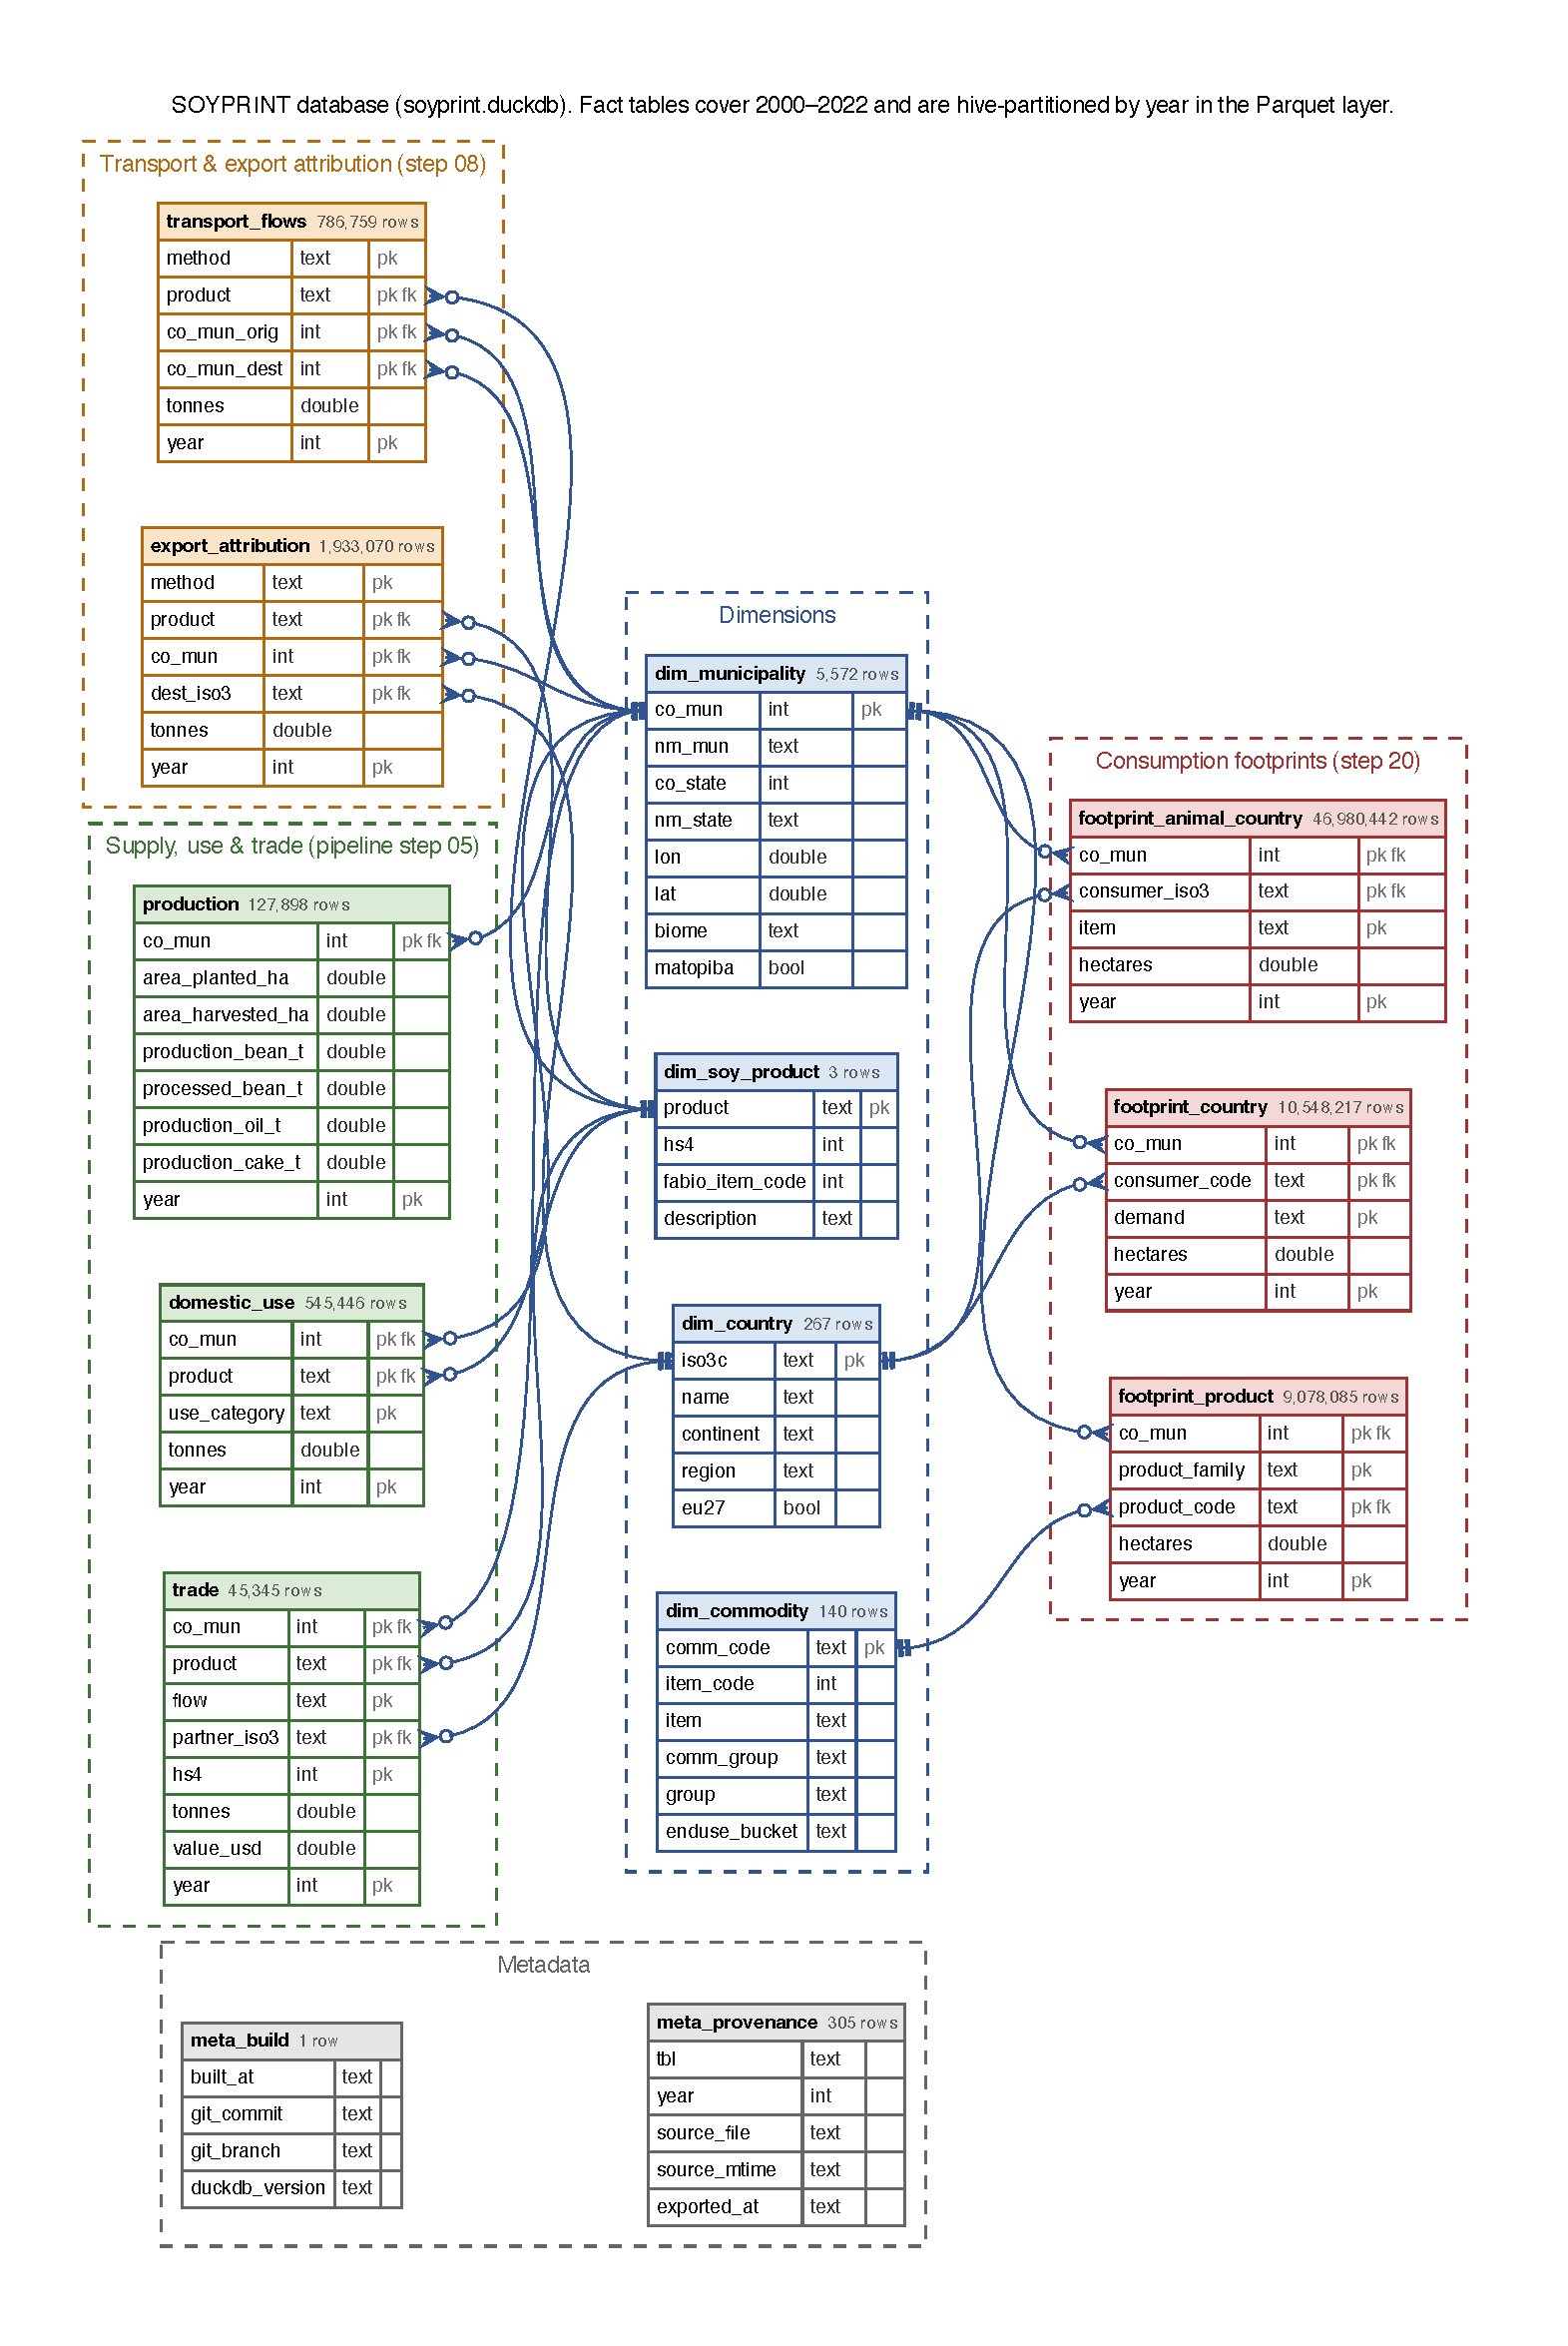
\includegraphics[width=\textwidth,height=0.88\textheight,keepaspectratio]{figures/fig_db_schema.pdf}
\caption{Schema of the released results database: eight fact tables,
grouped by the pipeline stage that produces them, linked to four
dimension tables, with build and provenance metadata alongside. Each
field is listed with its type, and primary and foreign keys are marked
(pk, fk). Fact tables are hive-partitioned by year in the Parquet
layer.}\label{fig:dbschema}
\end{figure}

\begin{figure}[H]
\centering
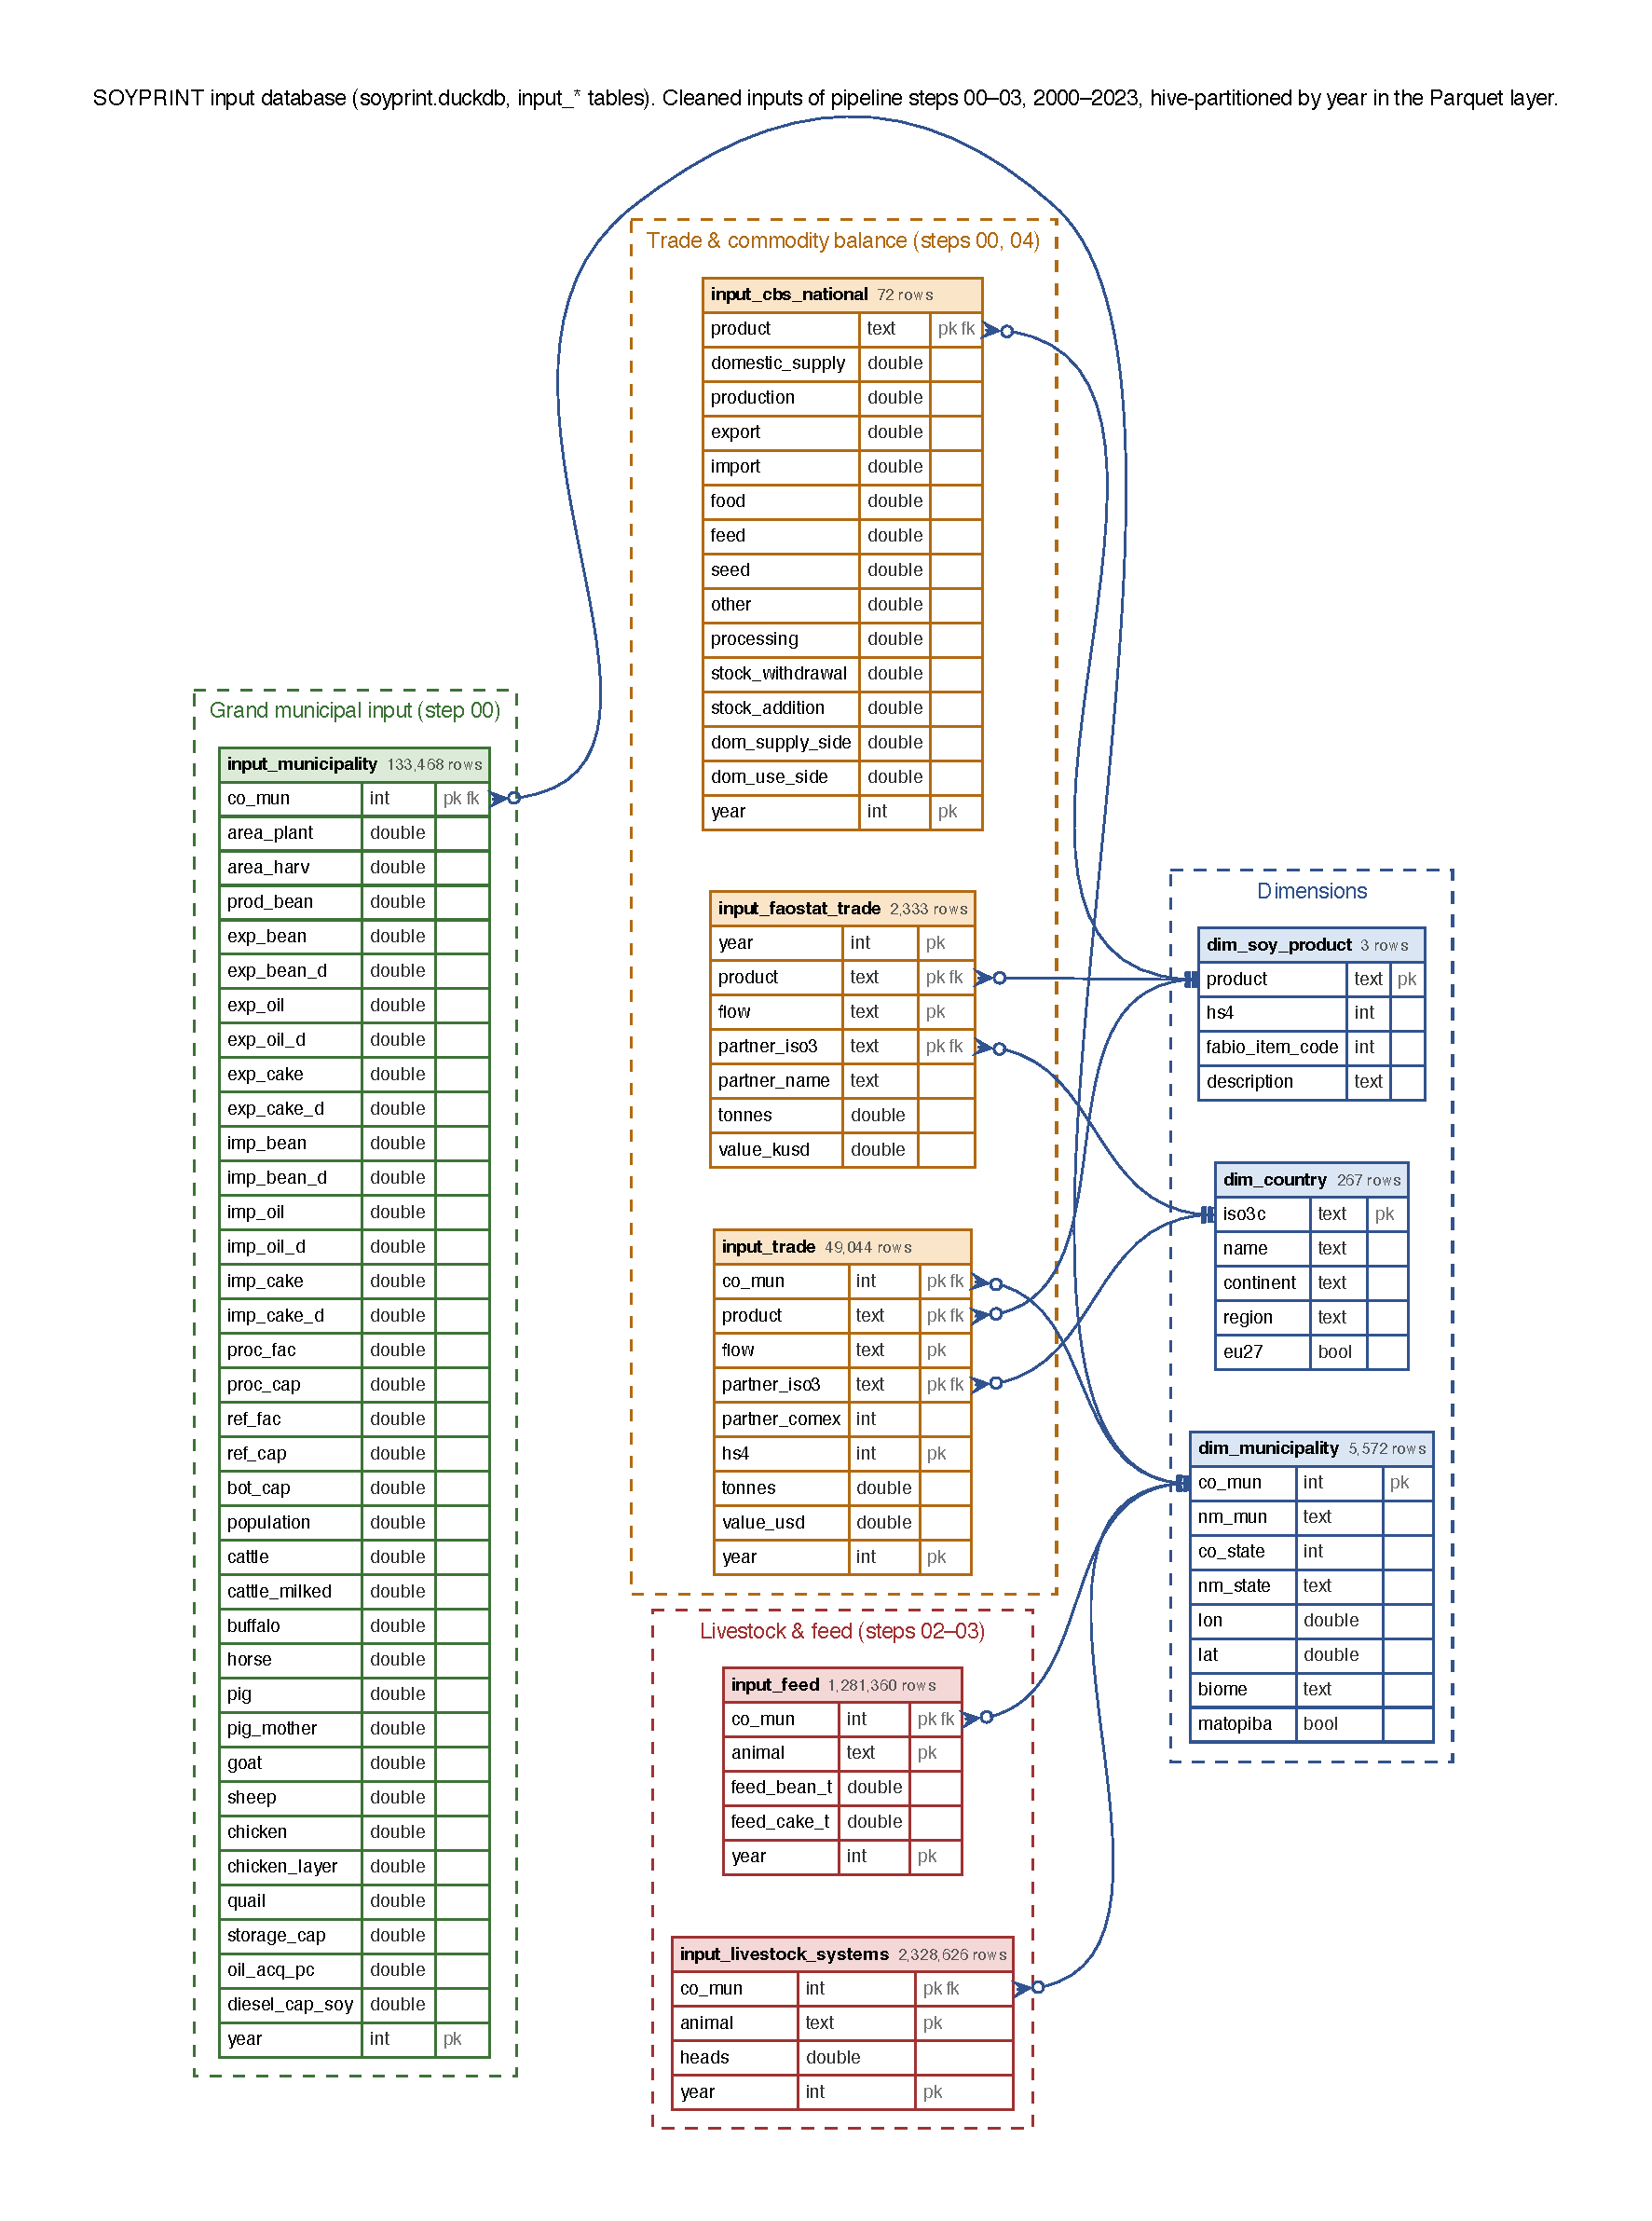
\includegraphics[width=\textwidth,height=0.88\textheight,keepaspectratio]{figures/fig_db_inputs_schema.pdf}
\caption{Schema of the input tables of the released database: the
harmonised inputs as the accounting stages consume them (the grand
municipal input,
the raw customs records, the national commodity balance, the FAOSTAT
bilateral benchmark, and the livestock-system and feed tables), linked
to the same dimension tables as the results. Each field is listed with
its type, and primary and foreign keys are marked (pk, fk). Like the
fact tables, the input tables are hive-partitioned by year in the
Parquet layer.}\label{fig:dbinputsschema}
\end{figure}

%%%%%%%%%%%%%%%%%%%%%%%%%%%%%%%%%%%%%%%%%%%%%%%%%%%%%%%%%%%%%%%%%%%%%%
\bibliography{refs}%
%%%%%%%%%%%%%%%%%%%%%%%%%%%%%%%%%%%%%%%%%%%%%%%%%%%%%%%%%%%%%%%%%%%%%%

\end{document}
